%-------------------------------------
%       Load document class
%-------------------------------------

\RequirePackage{calc}

\documentclass[
%   bibversion, % create the titlepage for the `Pflichtexemplare`
%   maxdis=3,   % number of pages before full form of abbreviation is used
%   font=lms,               % text font (lm: latin modern, lms: with serifs)
    minted,                 % use the minted package for code listings
%   infopath=/path/to/thesis_info,  % custom path to thesis information file
%   abstractpath=,          % custom path to abstract
%   zusammenpath=,          % custom path of the zusammenfassung
%   acknowledgmentspath=,   % custom path to acknowledgments
%   chapterstyle=veelo,     % change the appearance of the chapter titles
%   nominitoc,              % disable small TOCs at beginning of chapters
%   figlist,                % make a List of Figure
%   tablist,                % make a List of Tables
%   smallautoref,           % let autorefs have a small first letter
%   nostatistics,           % print no statistics on the bib page
%   bibtex,                 % use bibtex/natbib instead of biblatex/biber
%   noglossary,             % do not create an abbreviation list
    todo=margin,            % set type of todo notes (margin, plain, off)
%   fullcitename,           % show full first name in bibliography
    definitionindex,        % create index for definitions
%   smallmargins,           % reduce margin size and increase text width
%   baseonauthorstyle=gf,   % set the baseon authorstyle.
%   bibauthorstyle=fggf,    % set the biblatex authorstyle.
]{UniLeipzigBioinfThesis}

\makeatletter
% Define \titlegraphic to take one argument and do nothing.
% This overrides the broken call inside the class file.
\def\titlegraphic#1{} 
\makeatother

% Set the graphics path, i.e. the places where LaTeX will look for image files
% included with \includegraphics. You can specify multiple paths if you like.
\graphicspath{{graphics/}{graphics/chapter1/}}


%-------------------------------------
%       Add bibliography file(s)
%-------------------------------------
% Note that, with the bibtex option, only one bibliography file is supported,
% while biblatex/biber allows multiple bib files (e.g. one for each chapter).

\addglobalbib{misc/literature.bib}      % filename of the bibliography

%-------------------------------------
%       Additional packages & commands
%-------------------------------------
% Defining all custom commands in a dedicated file helps you to keep the main
% file clean. You can also load and configure additional packages there.

% misc/custom_defs.tex
% Defining all custom commands in a dedicated file helps you to keep the main
% file clean. You can also load and configure additional packages there.

%-------------------------------------
%       Additional packages
%-------------------------------------
% Here you can load other packages.

\usepackage{xspace}             % smart space after custom commands
% \usepackage[option1,option2]{coolpackage}


%-------------------------------------
%       Additional commands
%-------------------------------------
% Here you can define your own commands.

%%%%% Logical markup
% Commands to style logical elements of your text. Adapt to your preferences!
\renewcommand{\titlegraphic}[1]{\vbox{\centering #1}}
\newcommand{\species}[1]{\textit{#1}}       % species names in italics
\newcommand{\seq}[1]{\texttt{#1}}           % RNA/DNA sequence
\newcommand{\file}[1]{\texttt{#1}}          % file names
\renewcommand{\cmd}[1]{\texttt{#1}}         % executable code and commands
\newcommand{\prog}[1]{\textit{#1}}          % names of programs & packages
\newcommand{\email}[1]{\href{mailto:#1}{\texttt{#1}}} % email with mailto link
\newcommand{\quo}[1]{\enquote{#1}}          % quotation marks, dep. on language
\newcommand{\tblhead}[1]{\textbf{#1}}       % header of tables
\newcommand{\pkg}[1]{\texttt{#1}}           % LaTeX package
\newcommand{\clsopt}[1]{\texttt{#1}}        % LaTeX class option


%%%%% Abbreviations
% Common abbreviations that are never spelled out. For domain-specific
% abbreviations that should be added to the List of Abbreviations, use the
% \defabb command instead!
\newcommand{\vs}{\emph{vs.\@}\xspace}   % vs as in versus
\newcommand{\eg}{e.\,g.\@\xspace}       % e.g. (for example)
\newcommand{\zb}{z.\,B.\@\xspace}       % z.B. (zum Beispiel)
\newcommand{\ie}{i.\,e.\@\xspace}       % i.e. (that is)
\newcommand{\wrt}{w.\,r.\,t.\@\xspace}  % w.r.t. (with respect to)
\newcommand{\cf}{cf.\@\xspace}          % cf. (see/refer to)
\newcommand{\fivepr}{\ensuremath{5^\prime}\xspace}      % 5' (five prime)
\newcommand{\threepr}{\ensuremath{3^\prime}\xspace}     % 3' (three prime)
\defabb{ToC}{Table of Contents}
\defabb{UTC}{Coordinated Universal Time}
\defabb{DAG}{Directed Acyclic Graph}
\defabb{mFAS}{minimum Feedback Arc Set}
\defabb{SV}{Super Vertex}[Super Vertices]

%%%%% Math
% For custom operators and math commands.
% \DeclareMathOperator{\var}{Var}             % variance
% \DeclareMathOperator*{\argmin}{arg\,min}    % arg min


%-------------------------------------
%       Symbols & Categories
%-------------------------------------
% Here you can place your own symbols and categories, cf. the manual.

%%%%% Categories
\addSymbolCategory{C}{Cycle}
\addSymbolCategory{T}{Tree}

%%%%% Symbols
% \sym{C}{The circumference of a cycle.}
% \sym{\pi}[kreis]{The ratio of a circle's circumference to its diameter.}[C]

% End of misc/custom_defs.tex
 % custom definitions and packages go to that file


%-------------------------------------
%       Document body
%-------------------------------------

\begin{document}

\makefrontmatter

\beginmainmatter

% Include the chapters of the thesis as separate files from the chapters folder
% Uncomment the lines as you write the chapters.
\part{Introduction}
\chapter{Introduction}% Main chapter title
\label{Chapter1} % For referencing the chapter elsewhere, use \ref{Chapter1}

\section{Welcome}

Welcome to the manual of the Uni Leipzig Bioinf Thesis class. This class gives
a solid backbone for your thesis writing at the \quo{Institut für Informatik}
at the \quo{Universität Leipzig}. It can be used as it is without any further
configuration. However, many things can be configured. So hopefully it fits
your needs and your idea of design.

This template is designed to fulfill the requirements of the
\quo{Promotionsordnung Fakultät für Mathematik und Informatik} as it is in 2018
\citep{web:promotion,web:promotion2}. So in case of changes in the regulation
some parts of this work may not longer be suitable.

This class has many class options and also introduces some new commands that
can be used. So when you really want to use it you should at least read
\autoref{AppendixA} and \autoref{AppendixB}. However, I would recommend you to
read the complete manual so you get an overview how things work and how things
should be done. Also, the short overviews in the Appendix reflect not every
single aspect of the commands and options.

This manual is not an introduction to \LaTeX. The authors assume that you
already typeset a scientific work with \LaTeX{} before and that you do not
need an introduction to the basic commands. The typesetting of mathematical
formulas is not covered, either.

The use of this class is free and you can change things by yourself and
redistribute it if you like. However, if you use it and it makes your life
easier, I would appreciate it when you mention me in your acknowledgments.
Something short like: \quo{Thanks to Fabian Gärtner for the latex class of
this thesis.}

If something does not work as expected, something needs an update because of
some changes or you miss an option to modify the template feel free to write
me an email: \email{fabian@bioinf.uni-leipzig.de}.  I will see if I can help
you.

\subsection{Disclaimer}
Before we start, here is a little warning. At the time I made this template, I
was a PhD student.  I have tried to be as accurate as possible in everything
that is written in this manual,  and also in choosing its default options.
However, some people might disagree with me and there is not just one correct
answer but rather several possible options. So trust your supervisor more than
anything I have done here. Again if you get some feedback that something has
to change I would appreciate hearing from you such that I can include changes
in order to keep the template updated.


\subsection{This Manual}
This manual was itself created with the given
\pkg{UniLeipzigBioinfThesis} class. In the original download, the source
files contain the code of this manual so that you have direct examples how
things are done in this class. Of course, you will delete it in order to write
your own content in the files. However, before you do it you may have a look
at the content and keep the pdf file in a separate location such that you can
reread the manual. You can also download it again in order to see the original
sources.

The only difference between this source and the source of \file{manual.pdf}
is the class option \clsopt{minted} (see \autoref{sub:codehigh}) and
\clsopt{zusammenpath} (see \autoref{sec:germanabstract}) are set different.
This is done to make it compile and a offer good starting point without any
further changes.

\section{Double-sided Print}
This style only supports double-sided layout for the thesis. This is not a
lack of an option, this is done purposely.  When reading on a screen, it makes
more or less no difference if the document is single-sided or double-sided.
The difference is in the way it is printed.  A double-sided print is done such
that every sheet of paper is printed on both sides. This has only advantages.
It is closer to normal books and therefore more natural to read. It makes the
thesis thinner so that it is easier to handle. It saves you money because you
print on and tie less pages. The last and best reason is that it reduces the
waste of paper and makes the world a better place. I believe this is the
reason why we all write a thesis, to make the world a better place.


\section{File Structure}
This template splits the content of the thesis into various different files.
This helps you to keep your work organized and allows you to only compile the
parts that you currently edit. It also enables the automatic generation of
stand-alone documents from several parts of the work (e.\,g.\ the abstract),
which are formally required for the Dekanat when you hand in your thesis.
Other files provide the functionality of the class itself and need not be
changed.  Another set of files helps you to compile the thesis and store your
personal information.

The thesis itself is compiled from the file \file{main.tex} in the root
directory. In this file, the thesis class is loaded and basic configuration is
done. Especially, every path to another file can be changed here so that all
files can be moved or renamed if necessary. More details are given in
\autoref{sec:main}. Then, all the content from the subfolders is included and
compiled into a single document. The class itself is taking care of creating
the front matter and back matter for you. In addition to the main file, one
tex file for each stand-alone document created from the thesis content is
provided:
\begin{description}
    \item[\file{abstract\_sa.tex}:]
        The stand-alone abstract.
    \item[\file{curriculum\_scientiae\_sa.tex}:]
        The curriculum outlining your scientific career.
    \item[\file{publications\_sa.tex}:]
        The list of all your scientific publications.
    \item[\file{selbststaendigkeitserklaerung\_sa.tex}:]
        The declaration that you are the original author of all your thesis'
        content and that you have properly marked all citations.
\end{description}

The classes for the thesis and the stand-alone documents are defined in the
files \file{UniLeipzigBioinfThesis.cls} and
\file{UniLeipzigBioinfThesisSA.cls}, respectively. A style file,
\file{UniLeipzigBioinfThesisCommon.sty}, contains code that is shared by
both classes.  These classes make all commands and styles available to the tex
files. You should not edit these files unless you want to add a new feature or
have to fix a bug.

The files \file{Makefile} and \file{latexmkrc} help you to compile the
documents, as explained in \autoref{sec:compilation}.

The folders have thematically different content. The \file{frontmatter}
folder contains files that are used in the front matter (abstract,
acknowledgments,\dots), the \file{chapters} folder contains a single tex
file for each chapter of the main text. The \file{graphics} folder contains
the graphics for the figures of the thesis.  The \file{appendices} folder
contains a single tex file for each appendix.  The last folder is
\file{backmatter} which contains files that are used in the back matter
(\eg the Curriculum Scientiae).  The \file{misc} folder contains two data
files and a tex file. \file{literature.bib} is the \prog{BibTeX} file that
contains all works that you cited from. Your personal data and thesis
information like title, keywords etc., is stored in \file{thesis\_info.tex}.
File \file{custom\_defs.tex} is for all commands you may want to define
yourself, as well as for loading other packages you may want to use. It comes
with some commands already that you can use or change if you like.

Finally, \file{manual.pdf} contains a copy of this manual. You may want to
keep it for future reference.


\section{How to Compile It}%
\label{sec:compilation}

The short version: run \cmd{make} to compile everything, or \cmd{make
main} to only compile the thesis. Run \cmd{make watch} to continuously
compile the thesis as you write. If you have problems or want more
information, please read on.

As of release v2.0 of this class, the build system has been completely
rewritten. It now relies on \prog{latexmk}, a dedicated tool for compiling
\LaTeX{} documents that is taking care of all required steps, including the
execution of \prog{bibtex}, \prog{biber}, \prog{makeindex},
\prog{pdflatex} etc., in the right order and as often as necessary. It is
also more efficient than manually calling all these tools, because it
determines which files have changed and regenerates the output as necessary.
Furthermore, it offers file monitoring to automatically recompile the
document as soon as any changes to the source code are saved, as well as
cleaning procedures. Still, a \file{Makefile} is provided to allow calling
\prog{latexmk} with a single command without having to remember all the
options and paths. For more information on how to compile using the provided
\file{Makefile}, refer to \autoref{sub:make}.

\subsection{Configuring \prog{latexmk}}
With this template comes the file \file{latexmkrc}, which already contains
the required configuration for \prog{latexmk}. Separating the configuration
from the \file{Makefile} has the advantage that \prog{latexmk} can also be
called via any third-party \LaTeX{} development environment or editor without
further configuration. For example, the compilation feature of the
\prog{vimtex} plugin for the editor \prog{vim} works out of the box with
the provided files.


\subsection{Makefile}%
\label{sub:make}

The provided \file{Makefile} is divided into the sections \quo{Config} and
\quo{Rules}. Usually, you don't have to touch the rules at all, and
changing the configuration variables is only necessary when you rename the
main or stand-alone tex files.

To compile the thesis and all other stand-alone document, run \cmd{make
all} or simply \cmd{make} in the thesis directory. \cmd{all} is called
the (default) \emph{target}, \ie the object that is to be made. The
\file{Makefile} also defines several other useful targets:
%
\begin{description}
    \item[main:] Compiles the main file, \ie the thesis. The main file is
        by definition the first file listed in the variable
        \cmd{TEX\_FILES}. Running \cmd{make main} is the quickest
        way to compile only the thesis, omitting the stand-alone documents.
    \item[\emph{filename}.pdf:] Compiles (only) \file{filename.pdf} from
        source \file{filename.tex} for any file name.
    \item[clean:] Removes \emph{all} generated files, including the pdf files.
    \item[watch:] Watches for changes to any of the sources of the main file
        and re-compiles them as soon as any are detected.
    \item[watch-filename.tex:] Like \cmd{watch}, but watch
        \file{filename.tex} instead of the main file.
\end{description}
%
You can also set the path to \prog{latexmk} and additional command line
arguments in the \file{Makefile}. A few additional targets are provided for
development purposes:
%
\begin{description}
    \item[dist:] Make a tarball (\file{.tar.gz} archive) of the thesis
        directory. Target \cmd{clean} is executed first. The file name can
        be set by changing the value of variable \cmd{DIST\_NAME}. Set
        \cmd{DIST\_EXCLUDE} to prevent certain files or directories from
        being included in the archive.
    \item[changes:] Update \file{CHANGES.md} by converting
        \file{appendices/changes.tex} (\ie the version history) to MarkDown
        using \prog{Pandoc}.
    \item[html:] Generate HTML versions of \file{README.md} and
        \file{appendices/changes.tex} to update the website of the thesis
        template.\footnote{\url{%
        https://www.bioinf.uni-leipzig.de/intern/phd-thesis-class/}}
\end{description}

\subsection{Dependencies and Compiling at the Bioinf Institute}
To compile this template, you obviously need a \LaTeX{} distribution. Under
Linux, this is usually \prog{TeXLive}, which is available in the official
package repositories of any major Linux distribution. However, as the template
has many features, it also depends on many packages. The easiest way to
provide them all is a full installation of all \prog{TeXLive} packages. In
Fedora 36, this is done by installing package \pkg{texlive-scheme-full}
using \cmd{dnf}. In Ubuntu 22.04, install \pkg{texlive-full} and
\pkg{python3-pygments} with \cmd{apt}.  Also make sure that
\cmd{make} is available if you want to use the \file{Makefile}.  As of
2022, the computers at the Bioinformatics institute run varying versions of
Fedora. If the required packages are not installed on your machine yet, please
send a short email to the system administrator --- Jens will gladly help you
out.

Though this template has not been tested on Windows, you may have luck with
\prog{MikTeX} as well.


\section{The Main File}%
\label{sec:main}

The main file can be divided into two parts: the preamble and the document
body. In the preamble the class is loaded with the desired options. In the
document body, the actual content of the thesis is included from other tex
files.

\subsection{Preamble}
The first thing that is done in the preamble is loading the required classes.
This is done with \verb|\documentclass[]{UniLeipzigBioinfThesis}|.  Class
options can be added in the square brackets.  The possible options are spread
in the manual but all are marked with a margin note.

After this, you need to attach one or more bib files to you thesis this is
explained in \autoref{sec:bib}. You can also defined additional commands and
load other packages here if necessary.

\subsection{Document Body}%
\label{sub:body}

The document starts with the \verb!\makefrontmatter! command. This command
creates the complete front matter of the thesis. This includes the title page,
the dedication, the bibliographic description, the abstract, the German
abstract, the acknowledgments and \abb{ToC}. Make sure that your personal data
in file \file{thesis\_info.tex} is correct as it is used to generate the
front matter.

The main matter of the thesis start with the call of the
\verb|\beginmainmatter| command. The command starts the page numbering with
Arabic numerals. The main matter is composed of chapters. Every chapter is in
a separated file. This files then are included in the main file with the
\verb|\include| command. For more details on chapters, have a look at
\autoref{sec:chapter}. The only other elements in the main matter are the
parts.  Parts are described in more detail in \autoref{cmd:part}.

The next part is the appendix. To start this part use the
\verb|\beginappendix| command. It changes the chapter behavior and adds an
entry to the \abb{ToC}.  Every appendix is in an extra file. To add these
files, use the \verb|\include| command again. For more information, see
\autoref{sec:app}. The last command is then \verb|\makebackmatter|. This
command creates the back matter that includes the List of Xs, bibliography,
curriculum scientiae and the declaration.

\section{Base Settings}
\subsection{Margins}%
\label{opt:margins}

By default, the template uses relatively wide margins as defined by the
default settings of the \emph{Memoir} class. Though this may seem unusual
first, especially when you are used to a typical Word document, but it is
generally considered the more aesthetic choice by most typographers. It also
reduces the eye movement  compared to longer lines and thus can be read more
easily. However, when you have much to say, this can make your thesis very
large and heavy when printing. Thus, it could make sense to reduce the margin
size. This of course reduces the space for margin notes and I would not use
them with small margins. You can change to smaller margins with the class
option \clsopt{smallmargins}\indexdef{smallmargins}.

\subsection{Font}%
\label{opt:font}

The default font that is used in the tex files is Latin modern with serifs.
This is different to usual latex documents that use Computer modern with
serifs as default font, but the result is usually much better.   You can
change the font with the class option \clsopt{font}\indexdef{font}.  The
possibilities are shown in Table~\ref{tab:fontoption}.

\begin{SCtable}
  \captiont{Font values.}{The values that the class option \quo{font} can have.}%
  \label{tab:fontoption}
    \begin{tabular}{l l}
        \toprule
        \tblhead{Value} & \tblhead{Font used}\\
        \midrule
        lm  & Latin modern without serifs \\
        lms & Latin modern with serifs (default)\\
        cm  & Computer modern without serifs\\
        cms & Computer modern with serifs\\
        \bottomrule
    \end{tabular}
\end{SCtable}


\subsection{Chapter Design}%
\label{sub:chapterdesign}

There are many different possibilities for chapter page design. To change this,
use the class option \clsopt{chapterstyle}.\indexdef{chapterstyle}.  An example
of the possible designs is shown in
Figures~\ref{fig:veelo}--\ref{fig:wilsondob}. However, you could use any design
of the \emph{Memoir} class shown in \citep[P:383-396]{wilson2018memoir}. The
default value is the \emph{veelo} style, which has a mini \abb{ToC} within
each start page of a new chapter.


\begin{figure}
    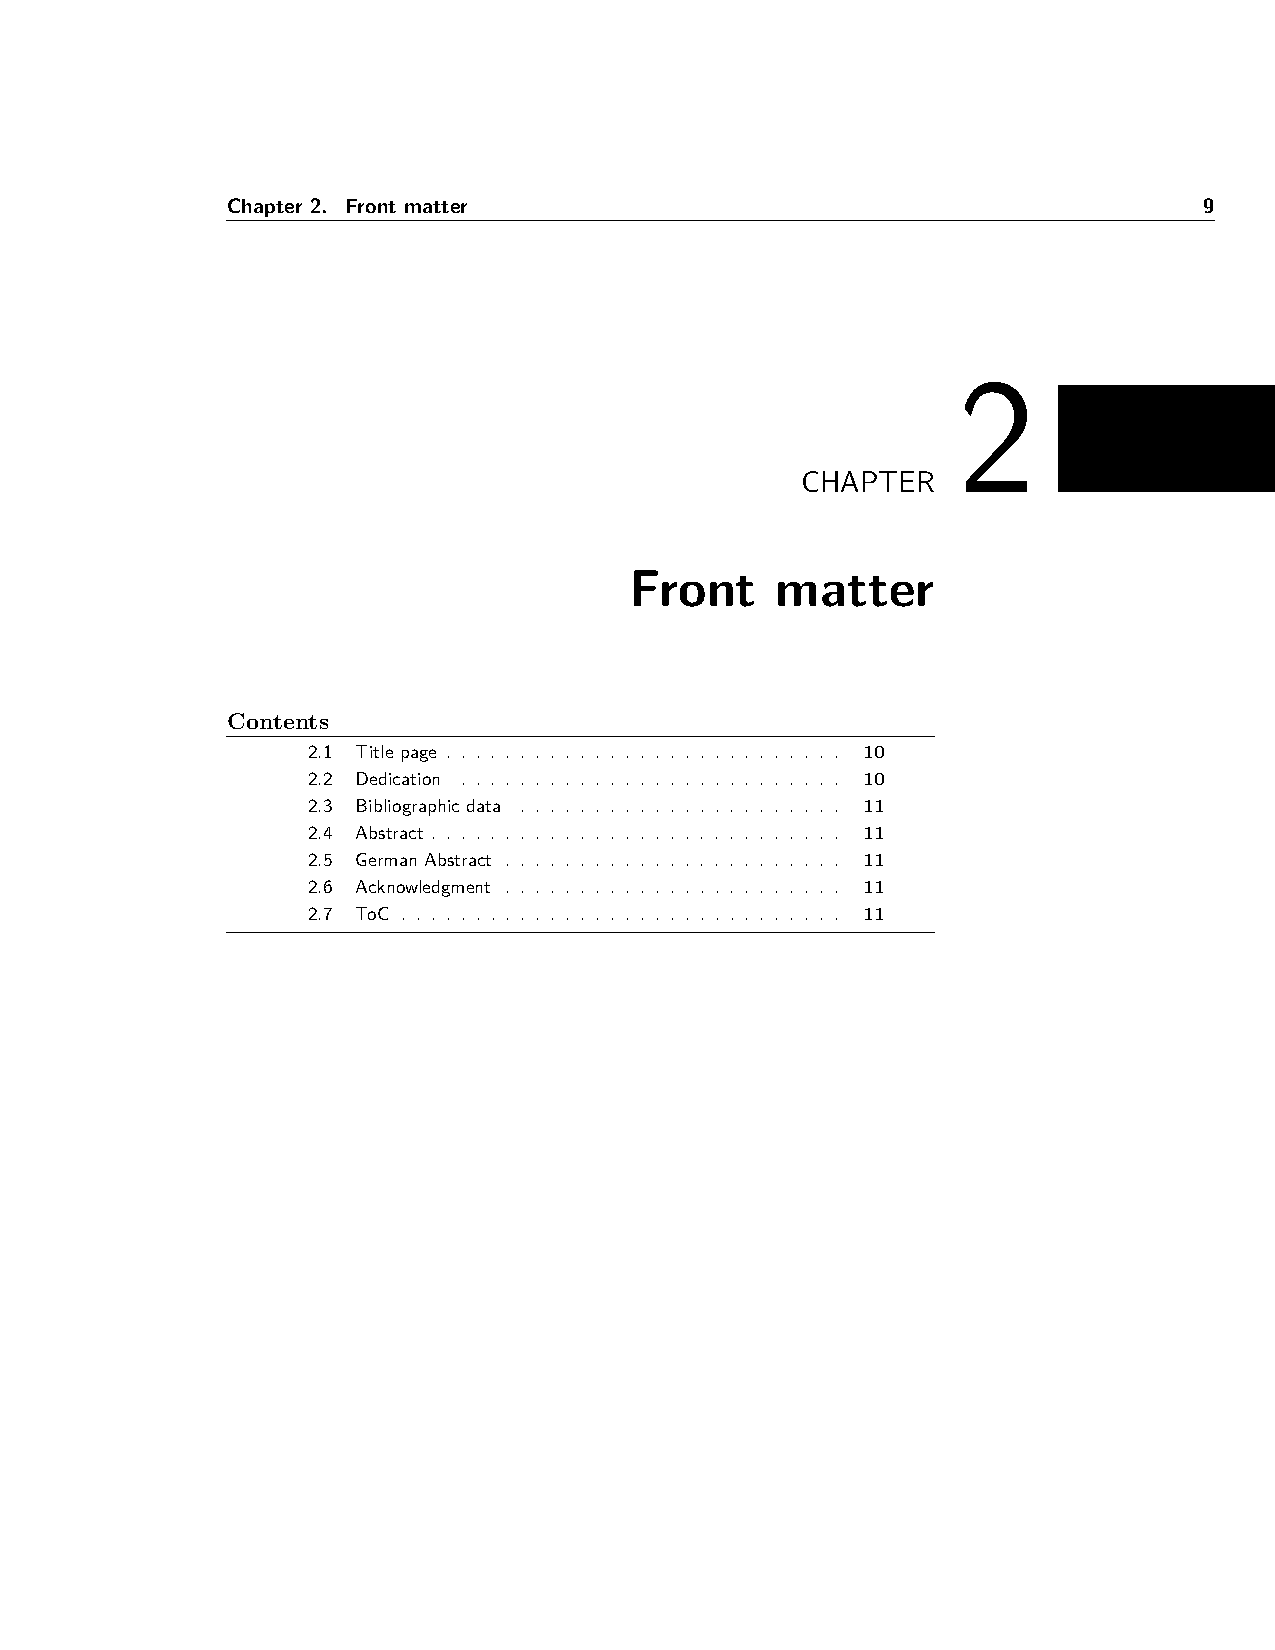
\includegraphics[scale=0.6]{veelo.pdf}
    \captiont{Veelo page style example.}{%
        An example how the veelo page style look with a mini \abb{ToC}}%
    \label{fig:veelo}
\end{figure}

\begin{figure}
    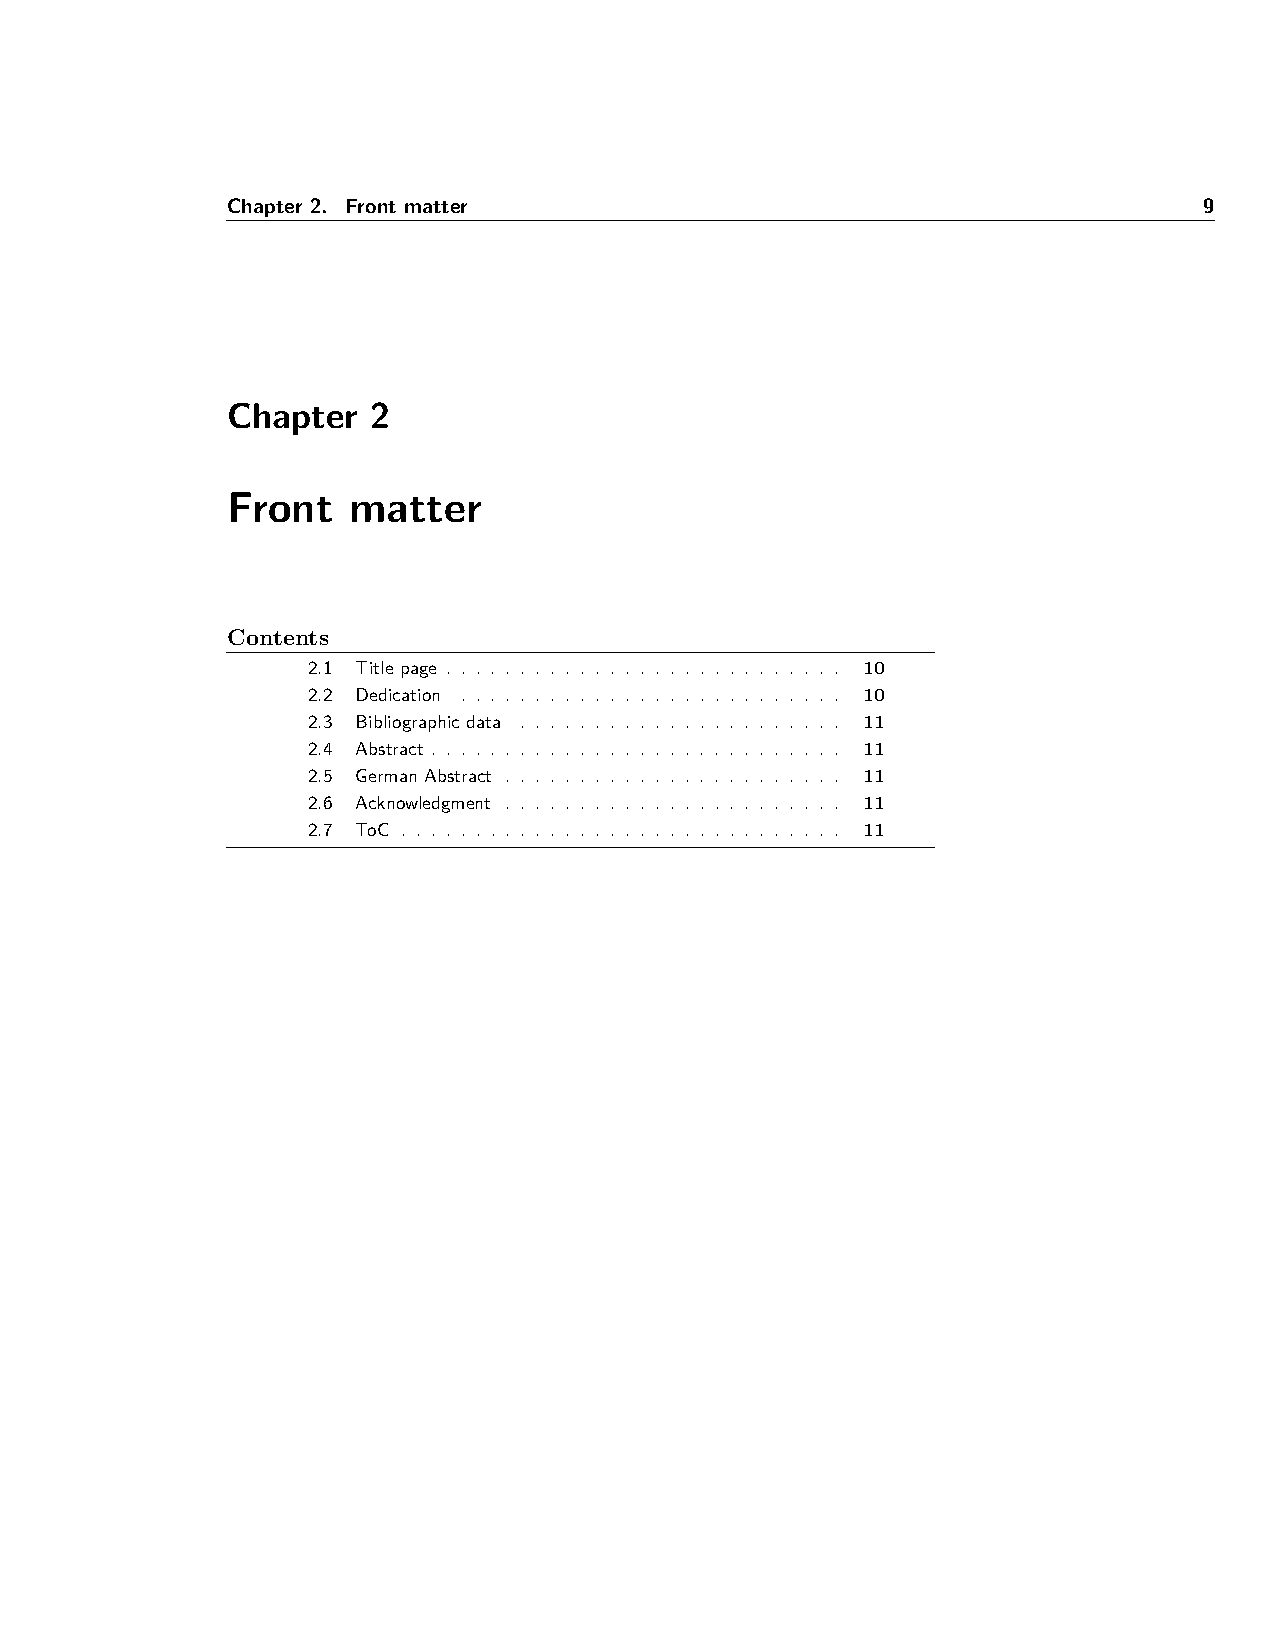
\includegraphics[scale=0.6]{default.pdf}
    \captiont{Default page style example.}{%
        An example how the default page style look with a mini \abb{ToC}}

\end{figure}

\begin{figure}
    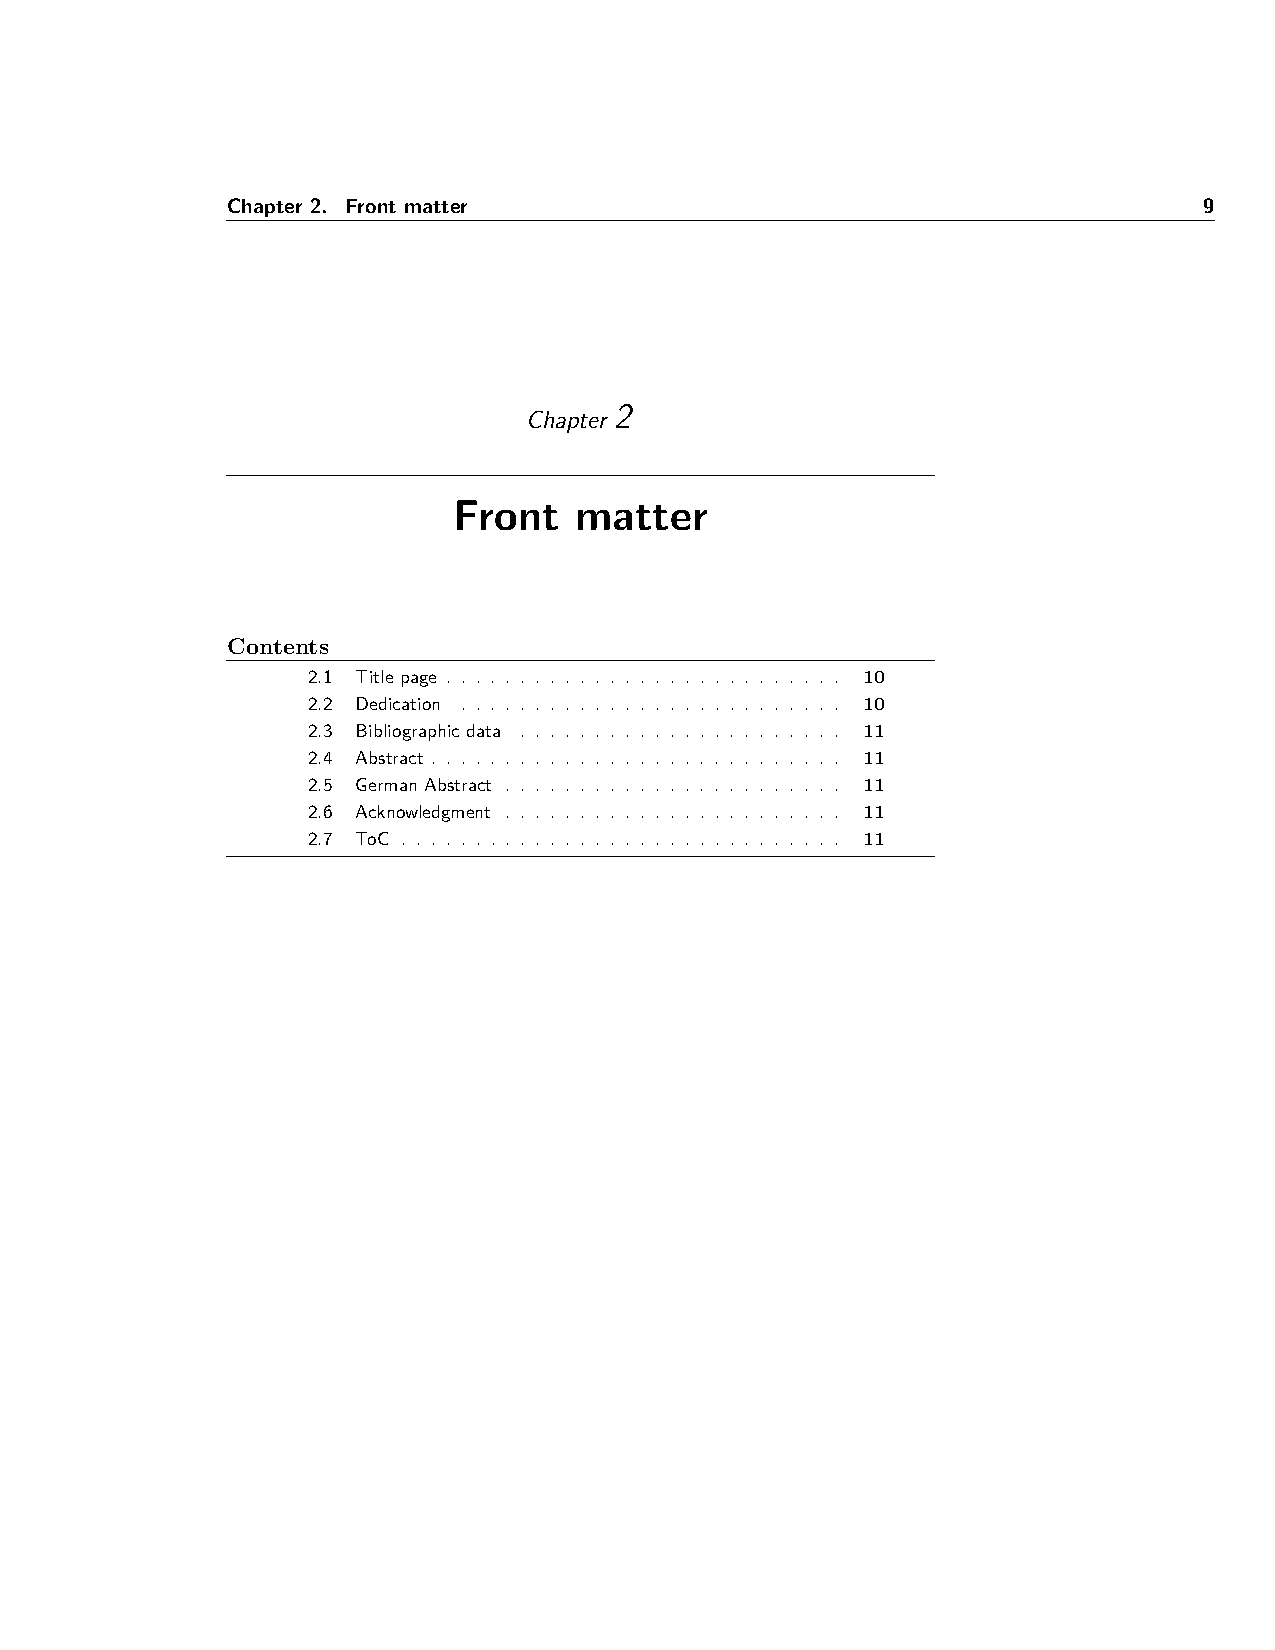
\includegraphics[scale=0.6]{bianchi.pdf}
    \captiont{Bianchi page style example.}{%
        An example how the bianchi page style look with a mini \abb{ToC}}
\end{figure}

\begin{figure}
    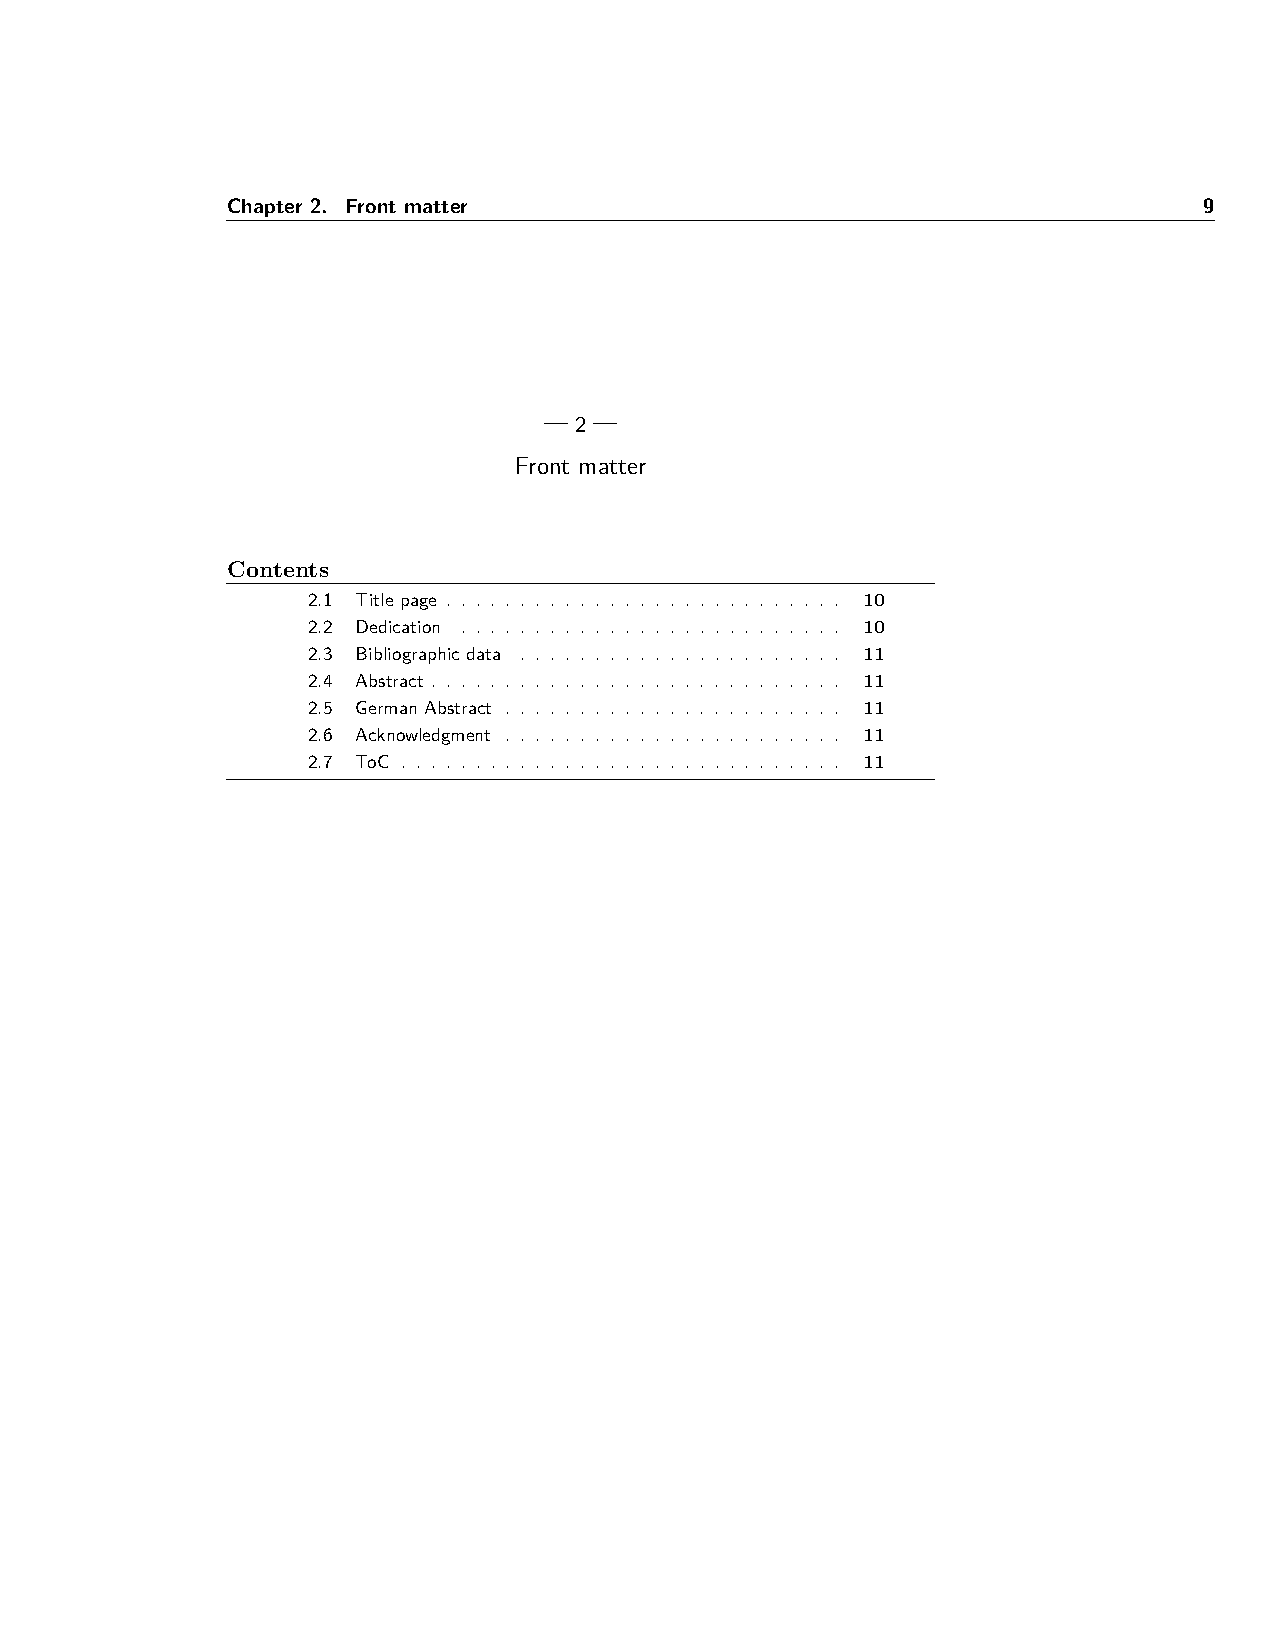
\includegraphics[scale=0.6]{dash.pdf}
    \captiont{Dash page style example.}{%
        An example how the dash page style look with a mini \abb{ToC}}
\end{figure}

\begin{figure}
    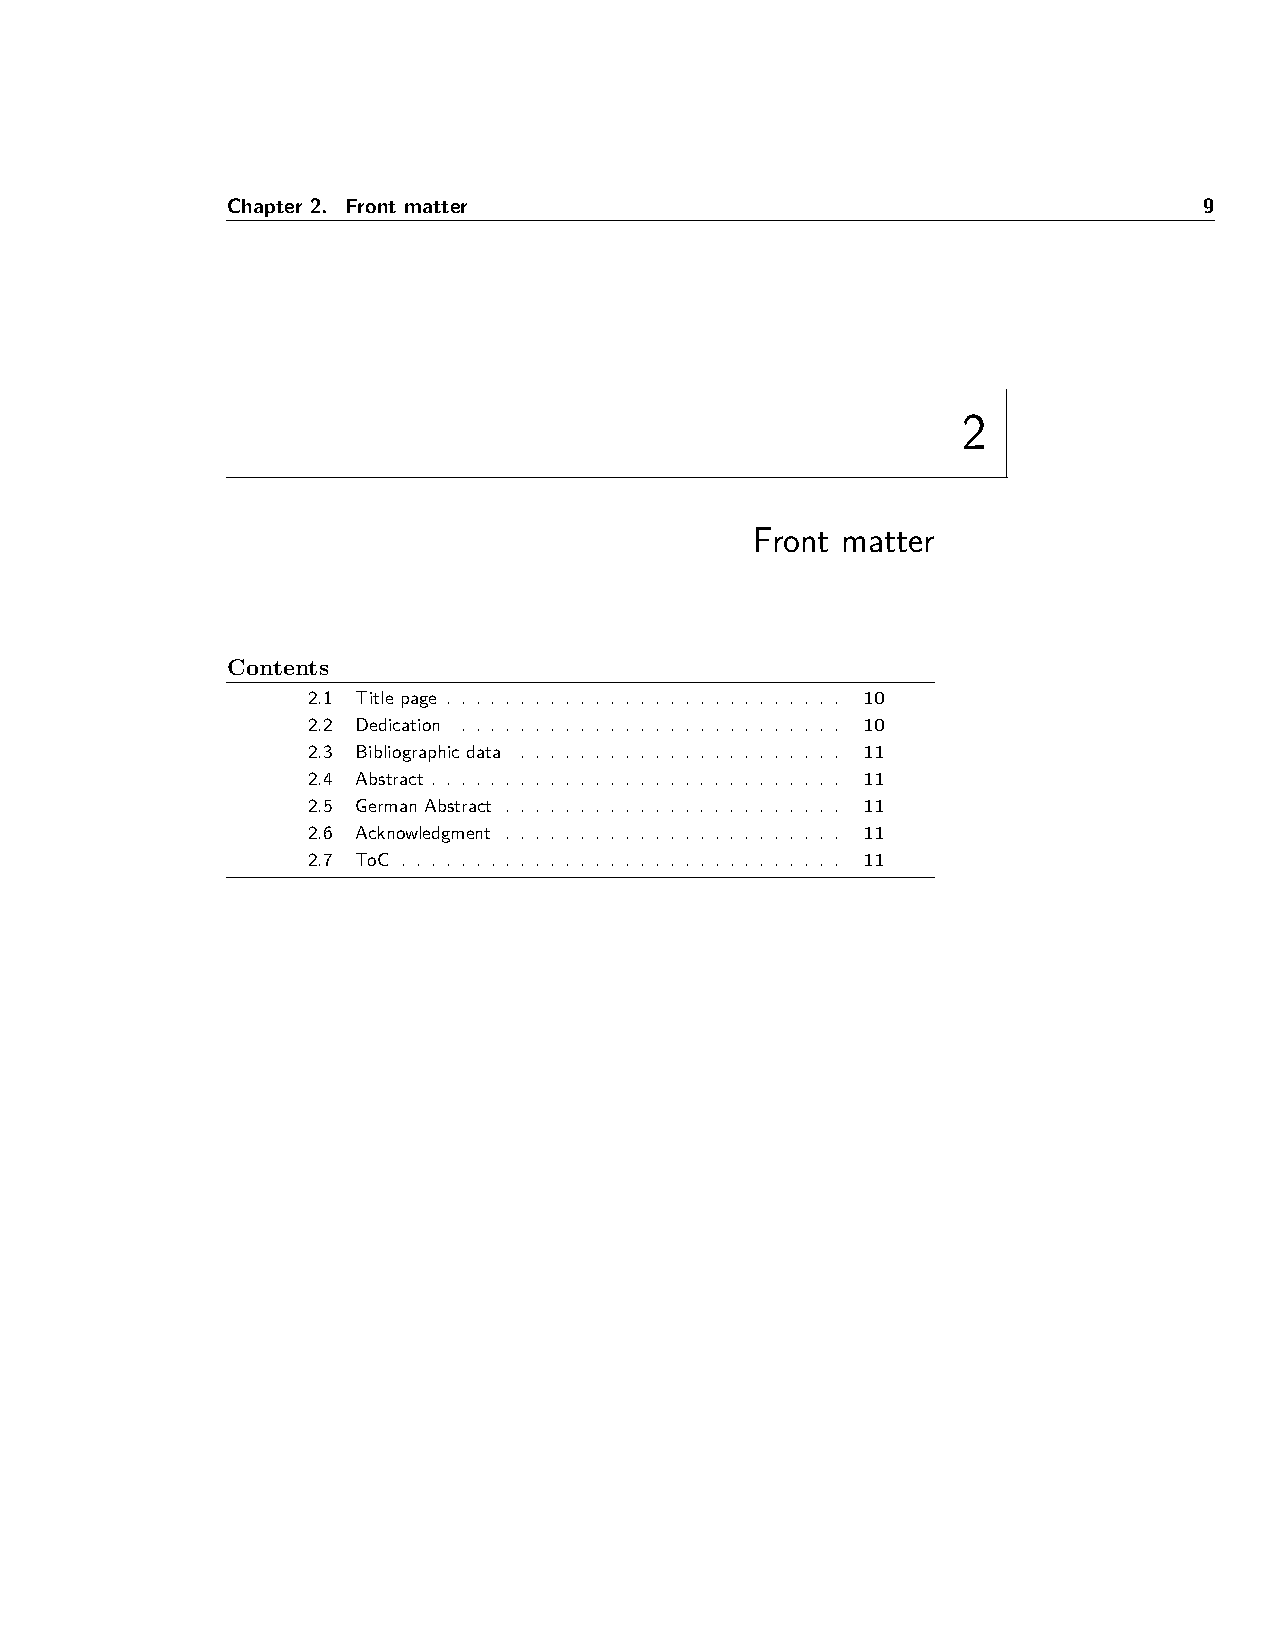
\includegraphics[scale=0.6]{ell.pdf}
    \captiont{Ell page style example.}{%
        An example how the ell page style look with a mini \abb{ToC}}
\end{figure}

\begin{figure}
    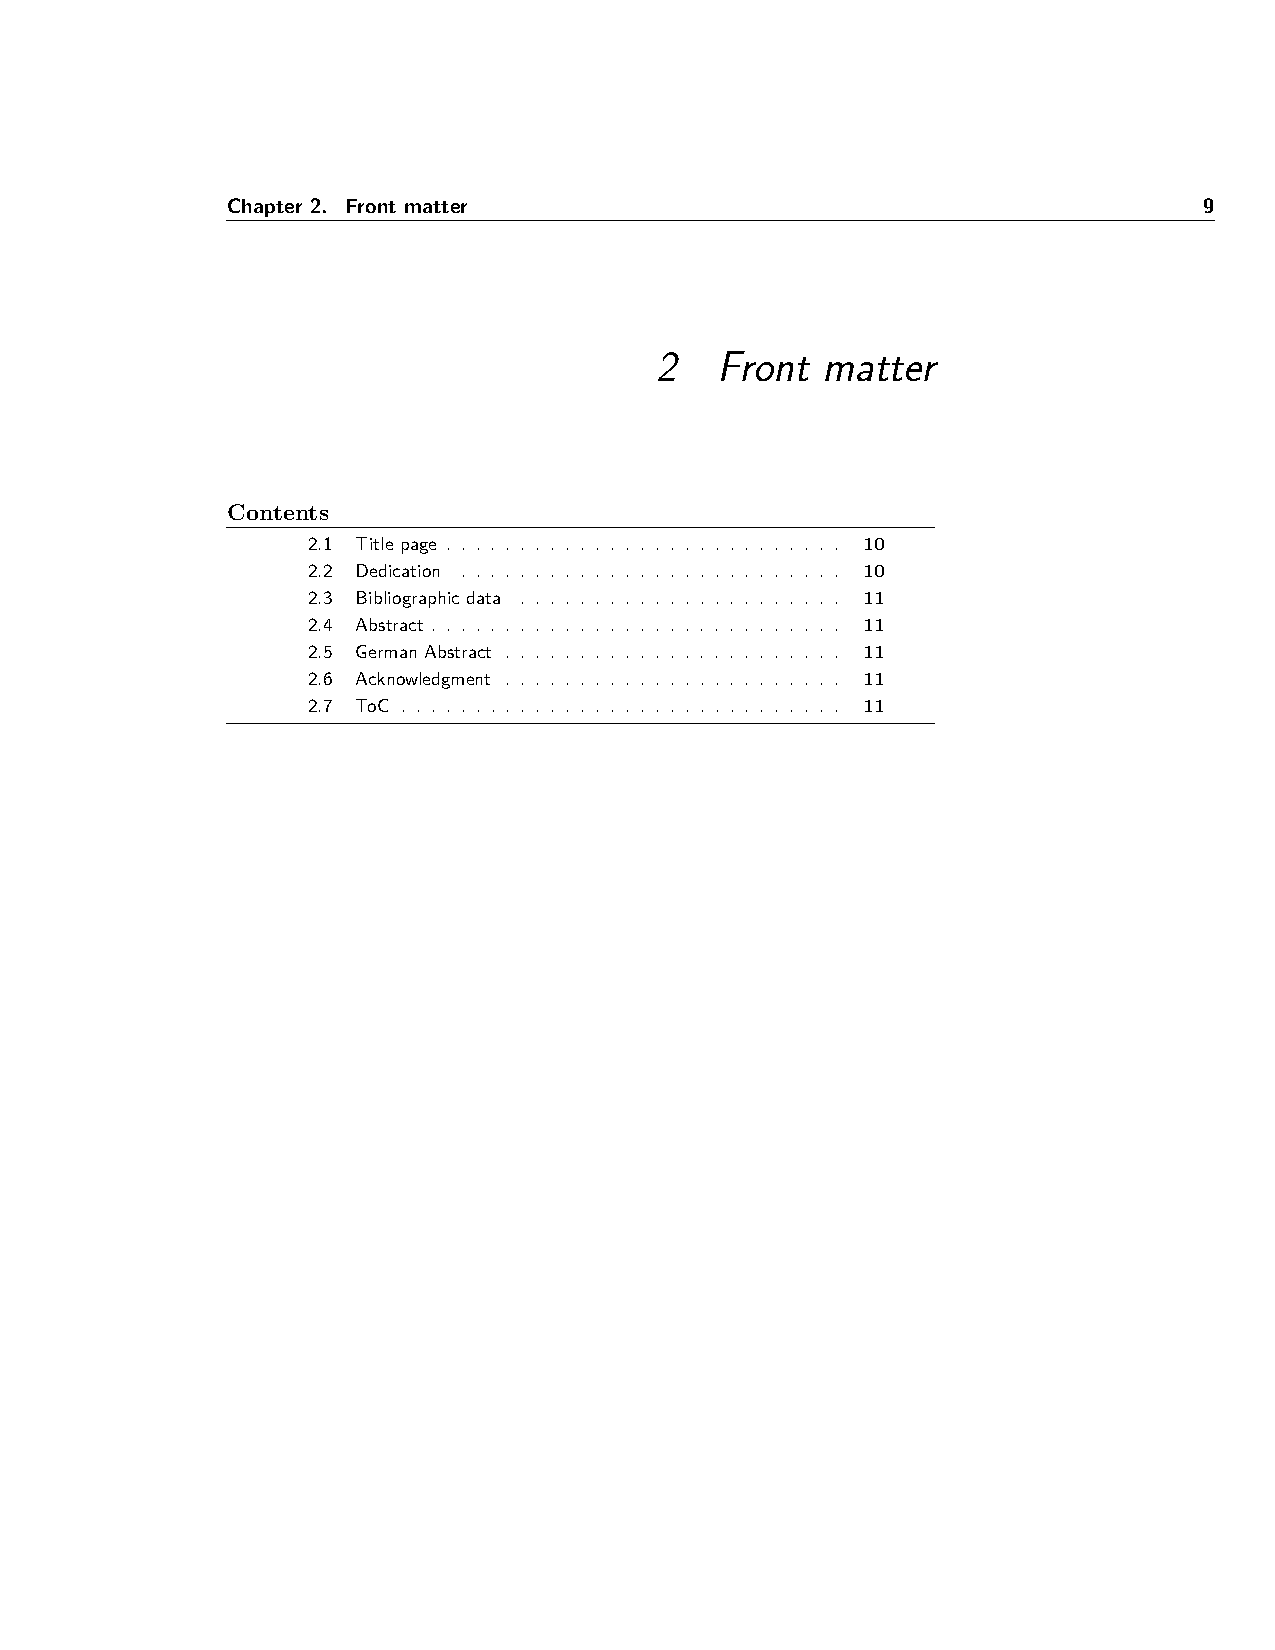
\includegraphics[scale=0.6]{wilsondob.pdf}
    \captiont{Wilsondob page style example.}{%
        An example how the wilsondob page style look with a mini \abb{ToC}}%
    \label{fig:wilsondob}
\end{figure}


\section{Common Typographic Mistakes}

While \LaTeX{} is designed to generate documents with a high typographic
quality, there are a few common pitfalls that authors have to be aware of to
avoid unexpected or unpleasant results. Here, some of the most relevant tricky
details to keep in mind are described.

\subsection{Logical Markup}
One of the most important rules to achieve a consistent typography in your \LaTeX{}
documents is to consequently use \emph{logical markup} like \verb!\emph! (for
emphasis) or \verb!\email! (for an email address) instead of directly styling
the text with low-level directives like, \eg, \verb!\textit! (for italic text)
or \verb!\tiny! (for small a font size). Logical markup means that you apply a
command to a piece of text that describes \emph{what it is}, and not what it
looks like. For example, a file name is often typeset in typewriter font.
However, instead of directly using \verb!\texttt{the_name}!  to achieve this,
it is better to define a command \verb!\file{}! for this purpose and use
\verb!\file{the_name}!. This has multiple benefits: (1) All file names using
this command will look identically, and you do not need to remember the exact
style. (2) You can easily change the style later by simply changing definition
of the logical markup command. (3) A custom command may be shorter than the
basic \LaTeX{} commands, especially if you have to use multiple ones to
achieve the desired look. (4) You can simply find all file names etc.\ in the
document by searching for the respective logical markup command. In case you
want to get rid of a logical markup command later, you can usually simply
replace all occurrences using a regular expression substitution.

To define your logical markup commands, use the \verb!\newcommand! command.
User-defined commands should be defined in file \file{misc/custom\_defs.tex}.
It already contains pre-defined commands for the most common text elements in
our fields, \eg \verb!\species! for species names, \verb!\prog! for computer
program names, and \verb!\cmd! for shell commands and code. For a complete
list, refer to \autoref{tab:logical_markup}. Of course, you can extend the
list or change the styles if you like.

\begin{SCtable}
    \centering
    \caption{%
        List of the default logical markup commands, which are defined in
        \file{misc/custom\_defs.tex}.
    }%
    \label{tab:logical_markup}
    \begin{tabular}{l l}
        \toprule
        \tblhead{Command} & \tblhead{Description} \\
        \midrule
        \verb!\species! & species name \\
        \verb!\seq!     & DNA/RNA sequence \\
        \verb!\file!    & file name \\
        \verb!\cmd!     & code or command \\
        \verb!\prog!    & program name \\
        \verb!\email!   & email address \\
        \verb!\quo!     & quotation marks \\
        \verb!\tblhead! & table headers \\
        \verb!\pkg!     & software package/module \\
        \bottomrule
    \end{tabular}
\end{SCtable}

\subsection{Spaces}
Inter-word spaces are a common source of typographic mistakes.  This is mainly
because, in \LaTeX, not every space has the same size. Most notably, it
increases the space after a period (\quo{\,.\,}), which is usually good as it
helps to visually separate different sentences. However, the period is also
used to mark abbreviations, which leads to wrong spacing as, \eg, in Mr. A.
Brown. The solution is to escape the following space, as in Mr.\ A.\ Brown
(using the code \verb!Mr.\ A.\ Brown!).

When defining a command which ends in a period, you do not know whether there
will be a space after it or not. In such cases, the sequence \verb!\@! can be
used to disable the increased size of a space that will possibly follow. For
example, \verb!\newcommand{\dr}{Dr.\@}! defines the command \verb!\dr!, which
is then displayed as Dr.\@ with correct spacing.

Beside regular spaces, \LaTeX{} also offers the command \verb!\,! to generate
half spaces. They are useful to group digits like 1\,500\,000 or to typeset
abbreviations consisting of multiple words like w.\,r.\,t.\ (\quo{with respect
to}), which looks much better than both w.\ r.\ t.\ (using full spaces) or
w.r.t.\ (using no spaces).

Another variety of the normal space is the \emph{unbreakable} space, written
as tilde character (\verb!~!). It has the same size as a regular space, but
prevents the line from being broken at this specific point. This is useful for
groups of text elements that belong together and should not be separated, for
example a title and a name like Mr.~Brown, or to prevent that abbreviations
followed by a period end a line and thus confuse the reader as it looks as
though the period ends the sentence.

A final recommendation is related to the somewhat surprising behaviour of
\LaTeX{} when it comes to spaces following commands. Using a command without
any arguments like \verb!\dr! defined above \quo{swallows} the following
space, \ie it will print Dr.and no space after it like so. To fix this, either
use \verb!\dr{}!, or use the \verb!\xspace! command from the \pkg{xspace}
package in the definition: \verb!\newcommand{\dr}{Dr.\@\xspace}!. It will
expand to a space only when needed and not, \eg, when used within parentheses.
The pre-defined markup commands in \file{misc/custom\_defs.tex} showcase the
use of \verb!\xspace!.

\subsection{Quotation Marks}

In short: always use the \verb!\quo{}! command to quote your text like
\quo{this}.

While using proper quotation marks like \quo{these} seems to be easy at a
first glance, it turns out to be a complex matter. First, one should realize
that the double quote character " looks horrid and should never be used in a
\LaTeX{} text. Instead, two backticks (\verb!``!) and two apostrophes
\verb!''! are used to create correct double quotation marks as in the first
sentence. Note how the opening and closing marks differ slightly. To make
things worse, quotation marks are language-specific, so in the German
Zusammenfassung, you would for instance use \glqq{}diese Art von\grqq{}
quotation marks.  Since this is easy to get wrong, this thesis class properly
sets up the language settings for the respective parts and provides the
command \verb!\enquote{text}! from the package \pkg{csquotes}, as well as the
shorthand \verb!\quo{text}!. Using this command is not only convenient and
guaranteed to produce correct results, it also handles edge cases like inner
and outer quotes: \quo{\quo{Hello,} he said.}

\subsection{Dashes}

Texts contain a wide variety of dashes---\ie horizontal lines---that have
different lengths depending on their function. To insert partial sentences
that could also be surrounded by commas or parentheses, or to append them as
if following a semicolon, the \emph{em-dash} (German Geviertstrich) is used.
It is named after the widest letter M.  In \LaTeX{}, it is typeset using three
dash characters (\verb!---!).  The first sentence of this section demonstrates
its usage. The shorter \emph{en-dash} (German Halbgeviertstrich), has half the
size of an em-dash. It can be typeset using two dashes (\verb!--!). It is used
to indicate ranges (\eg 10--15 minutes), or for compound nouns as in
Watson--Crick base pair or protein--protein interaction. The shortest dash is
the hyphen (German Viertelgeviertstrich), written simply as \verb!-! in the
code. It is used to hyphenate words at the end of lines, or for compound
adjectives like \quo{fast-growing} and sometimes for prefixes like in
\quo{re-evaluate}.

To get correctly sized minus signs, always set negative numbers in a math
environment: $-5$ (code: \verb!$-5$!) and not -5.

\subsection{Position Specifiers of Floats}

Do not overuse position specifiers of floats environments. For example, the
figure environment allows to pass the specifiers h (\emph{here}), t
(\emph{top}), and b (\emph{bottom}) as in \verb!\begin{figure}[htb]!. Do not
use them unless you have a good reason. Do not add them to all of your figures
by default. \LaTeX{} usually does a good job finding a suitable position on
its own. If you feel you have to add specifiers, do it when you are close to
finishing that chapter, when you have already included all other figures, or
you may get surprising results.

\subsection{Tables}

Instead of using \verb!\hrule! to draw horizontal lines in tables, use
\verb!\toprule!, \verb!\midrule!, and \verb!\bottomrule! as in the tables of
this manual, \eg~\autoref{tab:logical_markup}. Do not overuse these commands
as too many lines will only clutter your table, but not benefit its
readability.


% End of chapters/chapter_1.tex

\part{Content}
% Chapter 2

\chapter{Front Matter}% Main chapter title
\label{Chapter2}

\section{Title Page}%
\label{opt:bib}

The first page of the work is the title page. The design of this page is
specified by \citet{web:promotion}. There exist two versions of the title page
for different applications. The first one is the title page for your
submission of the thesis. After a successful defense of your thesis, it needs
to be published. This is done by uploading your work to
\url{http://ul.qucosa.de}. However, this version needs a different title page.
This is the second version of the title page. To create this title page
instead of the submission title page use the class option
\clsopt{bibversion}.\indexdef{bibversion}

The information on this page is provided by some commands in the data file
\file{thesis\_info.tex}. An overview of this commands is shown in
\autoref{tab:titlepage}. Note that most of the information exclusive for the
bib version can only be given after you defense. This is no problem because
you only need this version afterwards.

A little note to the \verb!\setsubtitle!: Not every work has or needs a
subtitle. In this case, you can simply not use the command
anywhere and the class eliminates the appearance of the subtitle everywhere.


\begin{table}
    \captiont{Titlepage commands}{%
        The commands that are used in the preamble of \file{main.tex} to
        input the information of the title page. Also is given if the
        information is used in the submission (sub) version or the bib
        version.
    }%
    \label{tab:titlepage}
    \begin{tabular}{l l l}
        \toprule
        \tblhead{Command} & \tblhead{Description}& \tblhead{Used for}\\
        \midrule
        \verb!\settitle!&The title of the thesis.&sub, bib\\
        \verb!\setsubtitle!&The subtitle of the thesis.&sub, bib\\
        \verb!\setauthortitle!&The academic degree if the author.&sub, bib\\
        \verb!\setauthor!&The full name of the author.&sub, bib\\
        \verb!\setdayofbirth!&The day of birth of the author.&sub, bib\\
        \verb!\setbirthplace!&The birth place of the author.&sub, bib\\
        \verb!\setfilingdate!&The date where you submit your thesis.&sub\\
        \verb!\setfirstreviewer!&The first reviewer of you thesis&bib\\
        \verb!\setsecondreviewer!&The second reviewer of you thesis&bib\\
        \verb!\setdayofdefens!&The day where you defended your thesis&bib\\
        \verb!\setgrade!&The grade that you get on your thesis&bib\\
        \bottomrule
    \end{tabular}
\end{table}


\section{Dedication}%
\label{cmd:dedicate}

The next page after the title page is the Dedication page. Here you can
dedicate your work to someone or make a suitable insider joke. Whatever it is,
it should be short and in the best case one sentence. You can input this
sentence with the \verb!\setdedication! command in the preamble of
\file{main.tex}.

If you do not want to dedicate your work to someone then leave the command
empty (\verb!\setdedication{}!). This eliminates the dedication page. Note
that the content of \verb!\setdedication! can be any latex command so it not
only possible to write text it could also include a picture or a combination
of both.

\section{Bibliographic Data}

The third nonempty page contains the bibliographic data of the thesis. This
is required by \citet{web:promotion}. Most of the data is calculated
automatically. The only exceptions are the keywords of the thesis which
are inserted by the command \verb!\setkeywords! in the preamble of
\file{main.tex}. The keyword should be given as a comma-separated list.

\subsection{Statistics}%
\label{sub:stats}

In the middle of the page are some automatically calculated value. These
values are the core of the bibliographic data. However, they are not mandatory
from the Promotionsordnung \citep{web:promotion}. Thus, you can deactivate
them with the class option \clsopt{nostatistics}\indexdef{nostatistics}.
Then nothing is calculated or shown, and only the keywords and the paper the
thesis is based on are displayed.

\subsection{Thesis Publication}%
\label{sub:baseon}

Most likely you have published already some of the results you present in this
thesis. Such a publication is then a publication on which the thesis is based
on. They can be divided from publications you only cited by the fact that in
some way you retell them in the thesis. This can even mean that long
paragraphs are equal between them and the text of the thesis.  This
information is critical to prevent the accusation of plagiarism. So this
publications belongs to the bibliographic data of the thesis.

To add publications there is the command \verb!\setbase! in the preamble used.
The command gets a comma-separated list of BibTeX keys. Then it automatically
fetches the full information out of your BibTeX file. However, this, of
course, means that this publication must be in the BibTeX file of the thesis.

The look of this paper can be influenced with the class option
\clsopt{baseonauthorstyle}\indexdef{baseonauthorstyle}. This change how the
authors are displayed. More details can be found at \autoref{sub:author}. The
default value is \quo{gf} which means that first the given name comes and then
the family name.

A second possibility to change the look of the author respectively give extra
information of the authors. This is done by annotations. A deeper look into
annotations can be found in \autoref{sub:annotation}. Two things are vary
handy here. First to mark authors that share a first authorship. This make it
possible to mark that you are a first author even when you are not on first
position. The second thing is the possibility to underline specific authors.
This is useful when you want to mark you in the papers. Maybe when you not on
first position or when you have changes your name by a marriage. Even when
both is not given a mark is a good idea to make the reader easy to spot you.

\section{Abstract}%
\label{opt:abstract}

Then the abstract of the work follows. This is limited to four pages
\citep{web:promotion}. The abstract is written in an extra file. By default
this file is placed at \file{frontmatter/abstract.tex}. You can change the
path to the abstract with the class option
\clsopt{abstractpath}\indexdef{abstractpath}. Note that you have to
\emph{omit} the \file{.tex} extension when defining an alternative value for
this option.

A stand-alone version of the abstract is generated automatically. You are
required to hand it in together with your thesis. It will be handed out during
your defense.

\section{German Abstract}%
\label{sec:germanabstract}

The template gives the option to include a German version of your abstract.
This is mandatory when you write a binational thesis. If you only write it for
the University of Leipzig you can choose if you want to include it. However,
most people add a German abstract.

The default path is \file{frontmatter/zusammenfassung} (omit the \file{.tex}
extension). Again you can change the path to the file that contains the German
abstract with the class option \clsopt{zusammenpath}\indexdef{zusammenpath}.
If you do not want the German abstract, you can simply set the class option to
an empty value (\verb!zusammenpath=,!).

\section{Acknowledgments}%
\label{opt:ack}

The third part of the front matter that inputs text from another path is the
acknowledgments. Here you should thank everybody that helped you with the
thesis: family, friends, supervisor, fellow students and maybe me.

The class option \clsopt{acknowledgmentspath}\indexdef{acknowledgmentspath}
changes the path to the file. The default path is
\file{frontmatter/acknowledgments} (omit the \file{.tex} extension).

\section{The Table of Contents}
The \abb{ToC} is directly in front of the main matter. It only contains
entries from the main matter and the back matter. The \abb{ToC} shows entries
down to the section level. Subsections are not shown here. However, they are
shown in mini \abbs{ToC} at the beginning of each chapter. More details on
mini \abbs{ToC} are given in \autoref{sec:chapter}.

% End of chapters/chapter_2.tex

% Chapter 3

\chapter{Main Matter}% Main chapter title
\label{Chapter3}

\section{Parts}%
\label{cmd:part}

The highest form of document division is \emph{part}. This division is not
required at all. However, you can use it to give you work some structure.
There should not be more than three or four parts in the complete thesis.
Typical cases would be:
\begin{itemize}
    \item I Background or Introduction
    \item II Methodology
    \item III Application
\end{itemize}
To start a new part the command \verb!\part{title}! is used. This creates a
part page where the title is shown. It also generates an entry in the
\abb{ToC}.  The parts are automatically numbered with roman numbers but have
no influence on other numberings.

\section{Chapters}%
\label{sec:chapter}

The most important document division is the chapter. A new chapter is started
with \verb!\chapter{title}!. This creates a chapter page and generates an
entry in the \abb{ToC}. How the chapter page is designed as described in
\autoref{sub:chapterdesign}. The chapters are numbered with arabic numbers.
All following sections and subsections are in the chapter and thus, have the
chapter number.  The header also contains the chapter information. Thus a new
chapter changes the look of the header.

Maybe at different locations, the name of the chapter should be different.
There are three positions: First the entry in the \abb{ToC}. Second, the entry
in the header of the page and third is the title on the chapter page. It is
possible to give for each of the three locations a different title. Different
title version can be useful as an example when the title is too long for the
header of the page. For this the \verb!\chapter! command has two optional
arguments.  The command \verb!\chapter[TOC][HEADER]{TITLE}! generates in the
\abb{ToC} the entry \quo{TOC}. In the header, it generates the entry \quo{HEADER}
and on the chapter page the entry \quo{TITLE}.

\subsection{Mini TOC}%
\label{opt:mintoc}

At the beginning of every chapter in the main matter, a mini \abb{ToC} is
printed. This contains all sections and subsections of the chapter. The
advantage here is that the reader gets an overview directly at the beginning
of each chapter and doesn't have turn back to look at the main \abb{ToC}.

However, this needs some space and some people say it is page flay. So you may
want to disable the mini \abb{ToC}. To do this, set the class option
\clsopt{nominitoc}.\indexdef{nominitoc} When the mini \abb{ToC} is disabled
the text of the chapter begins directly on the same page under the chapter
title.


\section{Labels and References}%
\label{cmd:ref}

For internal references, the \verb!\label{key}! and the \verb!\ref{label}!
commands are normally used. This is fine and also works for this class.
However, there is a second option: the \verb!\autoref{label}! command. The
difference is that \verb!\ref! only returns the number of the referenced
object, where \verb!\autoref! also returns a suitable prefix depending on its
type (e.\,g.\ figure, section etc.). An example is shown in \autoref{alg:ref}.

The upside is that the generated hyperlinks already start at the prefix, so
they can be clicked more easily. It also reduces the possibility of
referencing the wrong object.  In rare cases, it makes it easier to change the
type of a float or a section (from/to subsection) because you do not need to
change the type prefix for every reference.

The downside is that \LaTeX{} needs to know to every type and how it should be
named.  Also, referencing more than one object is possibly not useful. Every
element that is predefined by this class can be used here. As long you do not
introduce new floats or theorems, \verb!\autoref! is the simplest way to go.
In the manual, \verb!\ref! is only used to reference more than one object (see
\autoref{sub:chapterdesign}).

A question naturally arising when using \verb!\autoref! is: \quo{How is the
type prefix displayed?} Should the first letter be uppercase or lowercase? The
default in this template is that every type prefix is spelled with an
uppercase first letter.  However, this behavior can be changed with the class
option \clsopt{smallautoref}\indexdef{smallautoref}. When it is specified, all
type prefixes are written spelled with lowercase letters.

\begin{algorithm}
    \captiont{Referencing alternatives}{%
            The two referencing methods that create the same output.
        }%
    \label{alg:ref}
    \begin{code}{latex}
See Figure~\ref{fig:veelo}.
See \autoref{fig:veelo}.
    \end{code}
\end{algorithm}

\section{Citations}%
\label{sec:cite}

There are two main citation commands that you should use: \verb!\citet! and
\verb!\citep!.  \verb!\citet! is used when the citation is read as part of the
\textbf{t}ext (\ie when using the author name as a noun), \eg when
saying that the \pkg{biblatex} package was written by \citet{web:biblatex}.
\verb!\citep! is used when the entire citation is in \textbf{p}arentheses
(which should be the default case), \eg when simply saying that we use the
\pkg{biblatex} package \citep{web:biblatex}.

Depending on whether the \clsopt{bibtex} option is used for loading the class,
citations are provided by the \pkg{natbib} package based on \pkg{bibtex}
(\clsopt{bibtex} given), or with \pkg{biblatex} in the \pkg{natbib}
compatibility mode (\pkg{bibtex} \emph{not} given). Since \pkg{biblatex}
is more modern and robust, you should not specify the \pkg{bibtex} option
unless you have a good reason to do so. By default, the \cmd{author-year}
style is used. Thus, not a number but the author name and year is printed.
This is more informative than only giving a number that you have to remember
and look up in the list of references to know the author.  Though numbered
citations are more common in papers, you should consider that your thesis is
going to be a much bigger document and the bibliography may become huge.

\section{Margin Notes}%
\label{cmd:margin}

There is the possibility to print notes in the margin of the space. More
precisely on the outside margin of the page. These notes are very prominent
and seen easily but destroy the reading flow because they are outside of the
normal reading area. This can be used for information that should be easily
found but should not be used too often because then it loses its importance
and only disturbs the reading flow.

To do such a margin note use the command \verb!\marginnote{text}!. An example
is in this manual the class option. Every time the class options are presented
in different sections all over the manual, the command appears as a margin
note.  Thus, every time a new class option is introduced a margin note gives a
hint that it is presented here. This makes it possible to scan quickly for a
specific class option.

\section{Definition Index}%
\label{cmd:defindex}

One of the most popular uses of margin notes is to give a reader the position
of a definition. Then when a term is used the reader can easily find it and
check what it means. This concept can be extended by creating an index at the
end of the thesis where for every definition a  site is given where to find
it. Such that from anywhere in a large thesis fast the right position of a
definition can be found.

This can be archived with a special command. The template gives the
\verb!\indexdef{name}! command. This command creates a margin note with the
given name at the side. Further when the
\clsopt{definitionindex}\indexdef{definitionindex} class option is given an
entry in the Definition Index is created.

However, not every time you want to create an index you also want to create a
margin note. Thus, there are two different commands also given in to create
index entries. First the \verb!\indexnomn{name}! command. This command creates
an entry in the index but does not print anything at the position. It could be
combined with the \verb!\marginnote{text}! command to create different content
in the margin note and the index.

The second other command is \verb!\indexbf{name}!. This command also creates
an index entry and print \quo{name} in bold letters.  Thus, a highlighting of the
position is possible without the disturbing character of margin notes. It is
particularly useful when small margins are used.

\section{Abbreviations}%
\label{sec:abb}

% Abbreviation definitions look like this:
%   \defabb{UTC}{Coordinated Universal Time}
% But you should add them to misc/custom_defs.tex, not to the chapter content!
Every thesis uses abbreviations. An abbreviation can be a generally used term
like time zones (\abb{UTC}) or a topic-specific thing (\abb{DAG}) but also
very specific problem descriptions (\abb{mFAS} Problem). So it is necessary to
keep track of these abbreviations in a List of Abbreviations.  To add a new
abbreviation use the \verb|\defabb{short}{long}| command.

Besides this list, other things must be considered. If an abbreviation is
first introduced a long version must be given to explain the abbreviation. In
the following, only the short version is used. However, after some pages of
not using the abbreviation, it is useful to use the long version again so that
the reader gets a reminder what this abbreviation stands for.  Another thing
that must be considered is that sometimes the plural (\abbs{DAG}) of an
abbreviation is used (per default an \quo{s} is added to the end).

So the abbreviation engine gives more than the \quo{List of Abbreviations}.
It also gives the possibility to access earlier defined abbreviations with the
\verb!\abb! (for plural \verb!\abbs!) command. This returns the long version
with the short version in parentheses after the long version was not used on
the pages before. An example of the syntax can be found in \autoref{alg:abb}.

The default plural form with simply appending an \quo{s} is not always the
correct way to go (\abbs{SV}). For such situations, the alternate command form
\verb|\defabb[label]{short}[plural short]{long}[plural long]|
with the optional arguments \verb|plural short| and \verb|plural long| can be
used.  One is the short version in plural and the other the long version in
the plural. Note that it is possible to give only one of the two plural forms,
the other is then simply created by adding \quo{s}. The \verb|label| argument
allows to assign a label to the abbreviation such that it can be referred to
using \verb|\abb{label}|, which then still prints the supplied
short or long form.  With the two-argument command, the short form of the
abbreviation is itself used as the label. However, for complex abbreviations
including formatting and other commands, this is not possible.

\begin{algorithm}
    \captiont{The abbreviations engine.}{%
        An example definition of Abbreviation and the use of it. It is also an
        entry to the List of Abbreviations created.
    }%
    \label{alg:abb}
    \begin{code}{latex}
\defabb{DAG}{Directed Acyclic Graph}
The life is a \abb{DAG}.
%The life is a Directed Acyclic Graph (DAG).
Many \abbs{DAG} together create a \abb{DAG}.
%Many DAGs together create a DAG.
\defabb{SV}[SVs]{Super Vertex}[Super Vertices]
\abbs{SV}
%Super Vertices (SVs)
    \end{code}
\end{algorithm}

The default value of pages between two uses of \verb!\abb! before the long
version is printed again is 3. This can be changed with the \clsopt{maxdis}
class option.\indexdef{maxdis} A value of 0 means that only the first
appearance is printed with the long version all other occurrences have the
short version.

The functionality described here comes from the glossary package. It is a
large package. Thus, it makes sense not load it when you do not want any
\quo{List of Abbreviation} at all. This deactivation is done with the class
option \clsopt{nostatistics}.\indexdef{nostatistics} After the deactivation,
the abbreviation commands still exists but do different things. The
\verb!\defabb! command does nothing, the \verb!\abb! command simple print the
abbreviation, and the \verb!\abbs! command print the abbreviation with an
\quo{s} at the end. This behavior makes it possible to use them and then later
activate the glossary package again and have the full functionality with the
commands.

\section{Symbols}%
\label{sec:sym}

In the back matter, a List of Symbols is presented. To make this possible,
symbols need to be defined first.  To introduce a new symbol, use the
command \verb!\sym{symbol}{Description}!.  The symbol can then be used in a
mathematical environments as well as in text. It is also added to the List of
Symbols using the provided description.  An example is shown in
\autoref{alg:sym}. While symbols may be defined within the document body, \eg
directly where they are used for the first time, it may be more manageable to
maintain all definitions in \file{misc/custom\_defs.tex} to have them all in a
single place.

\begin{algorithm}
    \captiont{The sym command.}{%
        An example definition of Symbol. The result can be seen in the List of
        Symbols.
    }%
    \label{alg:sym}
\begin{code}{latex}
\sym{C}{The circumference of a cycle.}
\sym{\pi}[kreis]{Ratio of a circle's
    circumference to its diameter.}
We use the new cool symbol in math
$\symkreis = 3.14\dots$ and in text \symkreis.

\operatorsym{lca}[lca]{The last common ancestor.}
Let \symlca be the last common ancestor. When $v$ has
two children $u$ and $w$ then is $\symlca(u,w)=v$.
\end{code}
\end{algorithm}

This is some extra work for the \quo{List of Symbols}. However, this list
really helps the reader to understand complex formal definitions. It is also
very helpful for the writer. The list makes it easy to determine if a symbol
is used twice with varying meaning. This should be avoided, even in such a
complex work as a thesis.

The syntax is simple. The definition has an optional field in the middle that
defines a name: \verb!\sym{symbol}[name]{Description}!. This name can then be
used to reference back to the symbol using the command \verb!\sym*name*!. If
the name is omitted, the symbol itself is used as the name. This works only if
the symbol consists of regular letters, otherwise a name must be provided.

Sometimes you may want to define a custom math operator as a symbol. This can
be done by using the \verb!\DeclareMathOperator{\lca}{lca}! command in
\file{misc/custom\_defs.tex} (or another place in the preamble).  Then, you
can create a symbol using this operator. However, if you really want, you can
also define an operator symbol in the document body with the help of
the \verb!\operatorsym{symbol}[name]{Description}! command. Note that this
makes it necessary to use the \verb!\sym*name*! command to refer to the
operator. If you do not wish to have the \quo{sym} prefix, you need to declare
the math operator using \verb!\DeclareMathOperator{\lca}{lca}!.

The symbol engine has a problem with the \quo{$\vert$} symbol. However, this
can be fixed by not using direct \quo{$|$} but one of the two command
replacements: \verb|\vert| or \verb|\mid|. The first one is more or less the
same as \quo{$|$} and is used for example to get the absolute value of a number.
The second have more space around it and is used in constructive set
definitions.

\operatorsym{lca}[lca]{The last common ancestor.}[T]
\sym{\pi}[kreis]{The ratio of a circle's circumference to its diameter.}[C]
\sym{C}{The circumference of a cycle.}[C]

\subsection{Ordering and Categories}
The ordering of the symbols fellow normal the ASCII code
(+<1<:<A<\textbackslash<a). Note symbols define with \verb!\operatorsym! are
placed with \verb!\operator! at the beginning. Especially the fact that
\quo{\textbackslash} is placed between \quo{A-Z} and \quo{a-z} in the ordering is
often some way counterintuitive. To improve on this, you can customize the
order.

Both \verb!\sym! and \verb!\operatorsym! have an optional argument at the
end. This defines the ordering. It is important to note that every symbol for
which this last argument is given is placed behind every symbol without a last
argument.  Thus, it often only makes sense to give such an ordering argument
either to all symbols or to none. As an example if \quo{\symlca} should be
placed as lca in the ordering the definition should look like:
\verb!\operatorsym{lca}{The last common ancestor.}[lca]!.

Some times you want to group you symbols. This can be archived in two steps.
First you must define the groups in the preamble. This is done with
\verb!\addSymbolCategory{C}{Cycle}! command. The first argument must be a
\emph{capital letter} and the second argument the name of the category.
Second, first argument can then be used as last argument on the symbol
definition to get a element in the category. It is important to note that this
really only work with one capital letter. When more then one letter is given or
a small letter \LaTeX{} can not use the category. An example can be seen in
\autoref{alg:symcat}.

\begin{algorithm}
    \captiont{The symbol categories.}{%
        An example definition of Symbol categories. The result can be seen in
        the List of Symbols.
    }%
    \label{alg:symcat}
\begin{code}{latex}
%Categories can only defined in the preamble.
\addSymbolCategory{C}{Cycle}
\addSymbolCategory{T}{Tree}

\begin{document}
% Symbols can defined in the document body.
\operatorsym{lca}[lca]{The last common ancestor.}[T]
\sym{\pi}[kreis]{The ratio of a circle's
    circumference to its diameter.}[C]
\sym{C}{The circumference of a cycle.}[C]
\end{document}

\end{code}
\end{algorithm}

\subsection{Symbols with Parameters}
In many situations, you do not only have a symbol but also the symbols depend
on other things. An example would be the vertex set of a graph. There are at
least two different used notations for this $G.V$ or $V(G)$.  However, it
makes only sense when the graph (in this case $G$) is given. Thus a vertex set
symbol needs a place that can be changed.

This behavior is reached with the \verb!\macrosym! command. This command
defines a macro that can be used in the thesis and also generates an entry in
the list of symbols. Because this needs a name for the macro, its signature is
different than the other methods.

The command \verb!\macrosym{content}{name}[C]{d}[p1][p2]...!
creates the macro that is \verb!\sym*name*!. The content is what is printed.
It is given in latex macro form which means for the first parameter is \quo{\#1}
and the second \quo{\#2} and so on. The category (C) and description (D) are the
same as by the other commands. The command ends with a list of the parameters
that are used in the index. There are up to 5 parameters possible. When you
want a macro with four parameters you need to give four at the end of the
command.

\begin{algorithm}
    \captiont{The macro symbol command.}{%
        Some examples of macro symbols and how they can be used.
    }%
    \label{alg:symmac}
\begin{code}{latex}
%Let G be the 'graph' category.
\macrosym{V(#1)}{vertexset}[G]{The vertex set of $G$}[G]
\macrosym{E(#1)}{edgeset}[G]{The vertex edge of $G$}[G]
\macrosym{#1[#2]}{indsub}[G]{Creates induced subgraph of $G$
 with vertex set $U$ }[S][U]
%Let S be the 'set' category.
\macrosym{###1}{cardinality}[S]{The number of elements
in set $U$}[U]

When $D$ is a directed graph and $U\subset\symvertexset{D}$ and
$H=\symindsub{D}{U}$ have no cycles then is
$\symcardinality{\symedgeset{H}}\leq\frac{1}
{\symcardinality{U}(\symcardinality{U}-1)}$.
\end{code}
\end{algorithm}
%Let G be the 'graph' category.
\macrosym{V(#1)}{vertexset}[G]{The vertex set of $G$}[G]
\macrosym{E(#1)}{edgeset}[G]{The vertex edge of $G$}[G]
\macrosym{#1[#2]}{indsub}[G]{%
    Creates induced subgraph of $G$ with vertex set $U$ }[S][U]
%Let S be the 'set' category.
\macrosym{\##1}{cardinality}[S]{The number of elements in set $U$}[U]

\autoref{alg:symmac} creates this output:
\begin{quote}
    When $D$ is a directed graph and $U\subset\symvertexset{D}$ and
    $H=\symindsub{D}{U}$ have no cycles then is
    $\symcardinality{\symedgeset{H}}\leq
    \frac{1}{\symcardinality{U}(\symcardinality{U}-1)}$.
\end{quote}

\section{Floats}%
\label{sec:float}

There are three basic types of floats: figure, table and algorithm. Beside
this, there are two special types: SCfigure and SCtable. These are the same as
the floats without \quo{SC}. The difference is that in these floats the caption
is placed beside the figure (table). This can be used with narrow figures
(tables) to save space. An example of SCtable can be seen at
\autoref{tab:fontoption}.

\subsection{Figures}

The include \verb!\includegraphics! command of a figure needs the path to the
figure. The important part is that this path must be given relative to the
main.tex file. For an example is the picture veelo.pdf in the Figures folder
linked as \quo{graphics/ell.pdf} in every Chapter.


\subsection{Captions}%
\label{sub:cap}

The caption can be used with the normal \verb!\caption! command. Remember,
that the optional argument that sets the title on the \quo{List of \dots} page.
However, an alternative in this class is the \verb!\captiont! command that has
a second mandatory argument that sets the title and also writes it as bold at
the beginning of the caption. An example is shown in \autoref{alg:caption}.

All captions use a little smaller font than the rest of the text. This helps
to distinguish between text and caption of a float. This supports the reading
flow.

The caption is placed above or under the content of the float depending on the
position of the caption command. However, normally the figure caption should
be placed under the content, in a table above the content and in an algorithm
also above the content.

\begin{algorithm}
    \caption{%
        An example of how the \cmd{captiont} command can be used.
    }%
    \label{alg:caption}
    \begin{code}{latex}
\begin{SCtable}
    \captiont{Font values.}%
    {The values that the class option \quo{font} can have.}%
    \label{tab:fontoption}
    \begin{tabular}{l r}
        \toprule
        \tblhead{Value} & \tblhead{Used Font}\\
        \midrule
        lm  & Latin modern without serifs (default)\\
        lms & Latin modern with serifs\\
        cm  & Computer modern without serifs\\
        cms & Computer modern with serifs\\
        \bottomrule
    \end{tabular}
\end{SCtable}
    \end{code}
\end{algorithm}

\section{Code}%
\label{sec:code}

This template provides two different ways to typeset program code. One is
meant for code written in a real programming language and includes syntax
highlighting, the other is for pseudo-code that is more abstract than real
code.  These variants use the \cmd{code} and the \cmd{algorithmic}
environments, respectively.  However, in both cases, a surrounding
\emph{float}, which is automatically positioned and provides a caption that
can be labelled and referenced, is useful. This feature is available in form
of the \cmd{algorithm} environment, which then includes either a \cmd{code} or
a \cmd{algorithmic} environment. An example is shown in \autoref{alg:algo}.

\begin{algorithm}
    \caption{%
        Example of an \cmd{algorithm} float enclosing a
        \cmd{code} environment to display its own code.
    }%
    \label{alg:algo}
    \begin{code}{latex}
\begin{algorithm}
    \caption{%
        Example of an \cmd{algorithm} float enclosing a
        \cmd{code} environment to display its own code.
     }%
    \label{alg:algo}
    *code environment*
\end{algorithm}
    \end{code}
\end{algorithm}

\subsection{Pseudo Code}
To typeset pseudo code, the \pkg{algorithmic} package is used. See
\autoref{algo:algorithmic} for how the code looks like
For more details what commands exist, please have a look at the
manual.\footnote{\url{ftp://ftp.fu-berlin.de/tex/CTAN/macros/latex/contrib/algorithms/algorithms.pdf}}

\begin{algorithm}
    \caption{%
        The \cmd{algorithmic} environment can be used to typeset
        pseudo-code.
    }%
    \label{algo:algorithmic}
    \begin{code}{latex}
\begin{algorithmic}
    *pseudo-code*
\end{algorithmic}
    \end{code}
\end{algorithm}

\subsection{Real Code with Highlighting}%
\label{sub:codehigh}

The \cmd{code} environment is used to typeset code written in a real
programming language. Passing the name of a supported programming language,
\eg \verb!\begin{code}{python}!, allows the package to apply syntax
highlighting to the code. An example is given in \autoref{alg:code}.  Though
\cmd{code} environments can be used by itself to place the code exactly at the
given position, you should usually enclose it by an \cmd{algorithm}
environment to allow automatic positioning and provide a proper caption as in
\autoref{alg:algo}.

For code highlighting, two different packages are used. The default package is
the \pkg{listings} package. This is nice because it works out of the box on
any \LaTeX{} distribution. To achieve nicer syntax highlighting (with color),
another package is used: the \pkg{minted} package. It depends on the external
\prog{Python} program \prog{Pygments}. In order to use it, you need to install
them. More information on this can be found
online.\footnote{\url{https://github.com/gpoore/minted}} The manual is created
with \pkg{minted}.  To use \pkg{minted} instead of \pkg{listings} you set the
class option \pkg{minted}.\indexdef{minted}

However, which package you use does not have an influence on the environment
name, which is always \cmd{code}. This makes it possible to switch between
both options on the fly.

\begin{algorithm}
    \caption{An example how code highlighting works.}%
    \label{alg:code}
    \begin{code2}{latex}
\begin{code}{python}
    *code*
\end{code}
    \end{code2}
\end{algorithm}


\section{Math Environments}%
\label{sec:theo}

There are six different environments that belong to this class. They all have
their own uses. The explanations of them are taken from \citet{web:theorems}.


\subsection{Proposition}
A proved and often interesting result, but generally less important than a
theorem.
\begin{code}{latex}
\begin{proposition}
    *text*
\end{proposition}
\end{code}

\subsection{Definition}
A precise and unambiguous description of the meaning of a mathematical term.
It characterizes the meaning of a word by giving all the properties and only
those properties that must be true.
\begin{code}{latex}
\begin{definition}
    *text*
\end{definition}
\end{code}

\subsection{Corollary}
A result in which the (usually short) proof relies heavily on a given theorem
(we often say that “this is a corollary of Theorem A”).
\begin{code}{latex}
\begin{corollary}
    *text*
\end{corollary}
\end{code}

\subsection{Theorem}
A mathematical statement that is proved using rigorous mathematical reasoning.
In a mathematical paper, the term theorem is often reserved for the most
important results.
\begin{code}{latex}
\begin{theorem}
    *text*
\end{theorem}
\end{code}

\subsection{Lemma}
A minor result whose sole purpose is to help in proving a theorem.  It is a
stepping stone on the path to proving a theorem.
\begin{code}{latex}
\begin{lemma}
    *text*
\end{lemma}
\end{code}

\subsection{Proof}
Every Corollary, Theorem and Lemma must be proven. Thus, such an environment,
a Proof environment should follow.
\begin{code}{latex}
\begin{proof}
    *text*
\end{proof}
\end{code}

\section{Todo Notes}%
\label{sec:todo}

Often, some task is left undone and has to be finished later.  This should be
made visible in the thesis. The \verb!\todo{}! command is the solution to this
problem.  It creates a colored note containing the todo text.\todo{This is an
example of a todo note. Try changing the \clsopt{todo} option of the class and
see what happens.} The exact behaviour can be controlled with the class option
\clsopt{todo}, which can be set to any of the three values \emph{margin},
\emph{plain}, and \emph{off}.  The \emph{margin} setting creates orange boxes
located in the margin, keeping the layout intact and separating text and
tasks. Additionally, a list of all remaining tasks is generated and placed on
the first page of the thesis. This is probably the most elegant solution, but
relies on the external package \pkg{marginnote}.  The \emph{plain} option
simply inserts the task as red text, enclosed in brackets and with a smaller
font size than the main text. It has no external dependencies.  The value
\emph{off}, finally, allows to temporarily disable the output of todo notes
completely without deleting them.  This is useful for creating drafts of the
thesis that should not contain the note text.

% End of chapters/chapter_3.tex

% Chapter 4

\chapter{Back Matter}%
\label{Chapter4}

\section{Appendix}%
\label{sec:app}

There may be more than one appendix. Each appendix should be
thematically consistent. As an example, you could have one appendix for extra
tables and one for pseudocode. However, it directly depends on your topic and
how you present it. Still, the appendix should not be entirely unlinked to the
main text. A small mention like \quo{more data in Appendix X} is sufficient to
justify an appendix.

Every appendix starts with a \verb|\chapter| command. This command behaves
differently in the appendix than in the main text. The numbering uses letters
instead of numbers. Furthermore, the mini \abb{ToC} is not present here.
Generally, the formatting of such an appendix can be done more freely than in
the main text.  For example, one appendix could entirely consist of tables
without any text except for the captions.

\section{Lists of X}%
\label{opt:list}

There are four \quo{List of X} entries in the back matter. The first two are
abbreviations and symbols. More details on both can be found in
\autoref{sec:abb} and \autoref{sec:sym}.

The other two are figures and tables. Both are in some way standard in a
thesis.  However, the real usage of them is small. Do you know someone that
ever looked for a specific table or figure in these lists? So these two lists
are per default not present in the back matter. However, if you still want to
include them in the thesis, use the class options
\clsopt{figlist}\indexdef{figlist} (for figures) and
\clsopt{tablist} (for tables) \indexdef{tablist}.

\section{Bibliography}%
\label{sec:bib}

The bibliography is created from one BibTeX file. This file is given in the
preamble by the command \verb!\addglobalbib!. It can be changed to anything
else. In fact, the bibliography is created with biblatex, which also accepts
other input formats than BibTeX. For an overview look at \citet{web:biblatex}.

The use of \pkg{biblatex} means that the bibliography is not created with
\prog{BibTeX} but with \prog{Biber}. This tool should be contained in any
reasonably modern \LaTeX{} distribution. However, many editors do not use it
as default so you may need to change the configuration there.

The bibliography displays only those entries that are cited at some point in
the thesis (see \autoref{sec:cite}).  With respect to the base on publications
(see \autoref{sub:baseon}), it may be required to have some works in the file
that are not cited anywhere. Note that the bibliography is created for the
main text and the appendix, so by default all citations must be contained in
this single file. You can, however, include other bib files by adding more
\verb!\addglobalbib!  commands to the main \LaTeX{} file.

By default, the first names are shortened to the first letter. This behavior
can be changed with the class command
\clsopt{fullcitename}\indexdef{fullcitename}. When you use this command, the
result is that the full first names are shown in all citations. Note that in
many cases the downloadable \prog{BibTeX} files only contains the shorted
first name.  When some of the citations use shortened and some complete names,
the result will be an inconsistent look. To prevent this, use the command only
when all you BibTeX entries have full first names.

\subsection{BibTex}%
\label{sub:bibtex}

Even though BibLaTeX is more powerful than BibTex, there may be situations
where you want to use BibTex instead, e.\,g.\ if Biber is not available. For
this case, the class option \clsopt{bibtex} can be used.\indexdef{bibtex}
BibTex keeps more or less all features intact. The style of the bibliography
changes a little and the overall look is less pleasant.  The same holds for
the cite commands. Thus, I clearly recommend to use BibLaTeX. If you still
want to use BibTex, you must also adapt the latexmkrc file to properly
configure latexmk for using BibTex.  Be aware that author style and
annotations also does not work with BibTex.

\subsection{Author Style}%
\label{sub:author}

The author style is the way how BibLaTeX shows the author name in the
bibliography. This is set with the class option
\clsopt{bibauthorstyle}\indexdef{bibauthorstyle}.  There are basically two
options: first the given name, then the family name (\cmd{gf}); or first
the family name, then a comma, and then the given name (\cmd{fg}).

More natural is to have the given name shown first. However, this can be
disturbing when the  bibliography is sorted after the family names. Thus, your
brain may have a hard time to figure out where in the sorting you are. A
possible solution is a mixed version of the style. This third possibility is
to have the first author in \cmd{fg} order and all other authors in
\cmd{gf} order (\cmd{fggf}).

You can use any of the three bold strings to both authorstyle class options.
The based on bibliography (\clsopt{baseonauthorstyle}) uses the \cmd{gf}
order by default because the ordering of the papers in this smaller list is
not so important. The main bibliography (\clsopt{bibauthorstyle}) uses the
\clsopt{fggf} order such that most authors can easily be read but the ordering
of the bibliography can also easily be followed.

\subsection{BibLaTeX Annotations}%
\label{sub:annotation}

BibLaTeX has the possibility to add annotations to a bib entry. These
annotations must then be interpreted from the class. This thesis template
interprets three different author annotations. These are the
\cmd{underlinebase}, \cmd{underlineall}, and \cmd{firstauthor}.

\begin{algorithm}
    \caption{An example how to use author annotations.}%
    \label{alg:annotations}
    \begin{code}{latex}
@article{van2000art,
    title={The art of writing a scientific article},
    author={Van der Geer, J and Hanraads, JAJ and Lupton, RA},
    AUTHOR+an = {1=underlinebase,firstauthor;2=firstauthor},
    journal={J. Sci. Commun},
    volume={163},
    number={2},
    pages={51--59},
    year={2000},
}
@misc{web:promotion2,
    author = "{Fakultät für Mathematik und Informatik}",
    AUTHOR+an = {1=underlineall},
    title = "Erste Änderungssatzung zur Promotionsordnung Fakultät für
              Mathematik und Informatik",
    year = "2017",
    howpublished = "\url{http://db.uni-leipzig.de/bekanntmachung/
                          dokudownload.php?dok_id=5033}",
    note = "[Online; accessed 27-August-2018]",
}
    \end{code}
\end{algorithm}


First, it is important to know how author annotations are added. This is done
with an extra field, the \cmd{AUTHOR+an} field. Examples can be seen in
\autoref{alg:annotations}. The content of the field is a list of entries that
address the list of authors. Thus, every item in the list starts with an
author position (starting with 1). Then follows a \quo{=} and the actual
annotations, each separated by a \quo{,}. The list items are then separated with
a \quo{;}.

As an example, this field: \\
\verb|AUTHOR+an = {1=underlinebase,firstauthor;2=firstauthor}|\\
means that the first author is annotated with \cmd{underlinebase} and
\cmd{firstauthor}. The second author is annotated with
\cmd{firstauthor}. Not every position has to be annotated. Thus,
the field \\\verb|AUTHOR+an = {3=underlinebase}|\\ would also be valid.

Now to the meaning of annotations. The \cmd{underlinebase} and the
\cmd{underlineall} annotations do more or less the same thing. They
underline the author name. A convenient way to use this is to underline your
own name in every paper. This makes it easy for the reader to recognize your
work. The difference between these two commands is that \cmd{underlinebase}
only underlines the name in the \quo{based on} bibliography (see
\autoref{sub:baseon}) and \cmd{underlineall} also underlines it in the main
bibliography. You may choose the preferred style according to your taste.
Underlining in the based on bibliography is always a good idea. In the main
bibliography, the underlined references may be a little lost in all the other
ones that are not from you.  However, if you cite many papers that you have
done some work for but the thesis is not based on them, it could help to show
all the work you have done.

The \cmd{firstauthor} annotation is used to mark authors that share the
first authorship of a paper. In the main bibliography, this gives no extra
information that helps finding the work. However, in the based on
bibliography, the situation is different. Maybe you share the first authorship
of a paper, but you are not at the first position. Then you can use this to
make clear that this work is really from you. Thus, the annotation only
effects the based on bibliography. Furthermore, note that this annotation only
makes sense when more than one author is marked. In papers where only one
first author exists, the annotation shall not be used.

\section{Curriculum Scientiae}%
\label{sec:cs}

The Promotionsordung \citep{web:promotion} requires you to hand in a
curriculum scientiae with you work.  This is a curriculum vitae with a focus
on your scientific work. It is not stated how you hand it in but it makes
sense to make it a part of your thesis. To make it an extra file, some extra
commands are provided by the class.

The first one is the \verb!cscategory! environment. This gives you the
environment where you can put \verb!\csentry! in. For every topic (Education,
Working Experience, IT Knowledge and so on), a new \verb!cscategory!
environment is created. Thus, the title of the topic is given as an argument to
the \verb!\begin{cscategory}{title}! command. Internally, the environment
creates a tabular environment such that a \verb!cscategory! must be complete
on one page.  However, this can be composited by breaking one category
manually in parts. The second part should have a \quo{(continued)} (or
\quo{(ctd.)} for short) in the title.

The \verb!\csentry{left}{right}[secondline]! command has as a first argument a
text that is positioned left on the page. This could be a date of an
employment or a subcategory. The second one is then the text that is placed
right on the page.  This is could be a job description or some skills. When
one line is not enough to describe the entry, there is an optional third
argument that creates a second line on the right.

In case you want to create sub-entries for an entry, such as a grade for an
education or a project of an employment, this can be done with the command
\verb|\bull|. This command is used in the second or third argument of the
\verb!\csentry! command. An example of the complete example is given in
\autoref{alg:cs}.

\begin{algorithm}
    \caption{An example how a curriculum scientiae is created.}%
    \label{alg:cs}
    \begin{code}{latex}
\begin{cscategory}{Working Experience}
    \csentry{since 10/2018}{Tutor}[
        Institute for Computer Science, Leipzig University
        \bull{} Lecture: Algorithms and Data Structures
    ]
\end{cscategory}
    \end{code}
\end{algorithm}

\section{Selbstständigkeitserklärung (Statement of Authorship)}
The last thing that is required by the Promotionsordung~\citep{web:promotion}
is that you sign a Statement of Authorship. This is the last page of your
thesis.  It basically says that you have done no plagiarism.

There are two lines. The first one is for the location and date where you
signed it. The second one is for your signature.

% End of chapters/chapter_4.tex

% New chapters can be included like this:
% \include{chapters/chapter_5}

\beginappendix

% Include the appendices of the thesis as separate files from the Appendices
% folder.  Uncomment the lines as you write the Appendices
% Appendix A

\chapter{Class Options Overview}%
\label{AppendixA}

\noindent
\begin{tabularx}{\linewidth}{l X l}
    \toprule
    \tblhead{Class Option} & \tblhead{Description} & \tblhead{Reference}\\
    \midrule
    abstractpath&The path of the abstract file&\autoref{opt:abstract}\\
    acknowledgmentpath&The path of the acknowledgment file&\autoref{opt:ack}\\
    baseonauthorstyle&Change the author style in based on bibliography&\autoref{sub:author}\\
    bibauthorstyle&Change the author style in main bibliography&\autoref{sub:author}\\
    bibversion&Create the bib version title page&\autoref{opt:bib}\\
    bibtex&Use BibTex instead of BibLaTeX&\autoref{sub:bibtex}\\
    chapterstyle&Change the appearance of the chapter title page&\autoref{sub:chapterdesign}\\
    definitionindex&Add a Definition Index&\autoref{cmd:defindex}\\
    figlist&Add a List of Figures&\autoref{opt:list}\\
    font&Change the font&\autoref{opt:font}\\
    fullcitename&Use full names in bibliography&\autoref{sec:bib}\\
    infopath&The path of the thesis information file&\autoref{opt:bib}\\
    maxdis&After how many pages the full version of a abbreviation is used&\autoref{sec:abb}\\
    minted&Use the minted package for code highlighting&\autoref{sub:codehigh}\\
    \bottomrule
\end{tabularx}

\clearpage

\noindent
\begin{tabularx}{\textwidth}{l X l}
    \toprule
    \tblhead{Class Option} & \tblhead{Description} & \tblhead{Reference}\\
    \midrule
    noglossary&Deactivate abbreviations commands&\autoref{sec:abb}\\
    nominitoc&Deactivate the mini toc&\autoref{opt:mintoc}\\
    nostatistics&Deactivate the statistics of the Bibliographic Description&\autoref{sub:stats}\\
    smallautoref&Change autoref typs to small letters&\autoref{cmd:ref}\\
    smallmargins&Change to small margins&\autoref{opt:margins}\\
    tablist&Add a List of Tables&\autoref{opt:list}\\
    todo&Aktivate todo notes&\autoref{sec:todo}\\
    zusammenpath&The path of the German abstract file&\autoref{sec:germanabstract}\\
    \bottomrule
\end{tabularx}


% End of appendices/appendix_A.tex

% Appendix B

\chapter{LaTeX Commands in the Class}%  % Just don't use \LaTeX in a caption..
\label{AppendixB}

\section{Preamble Commands}

\noindent
\begin{tabularx}{\linewidth}{l X l}
    \toprule
    \tblhead{Command} & \tblhead{Description} & \tblhead{Reference}\\
    \midrule
    \verb|\addglobalbib|&Add a bib file&\autoref{sec:bib}\\
    \verb|\addSymbolCategory|&Add a Symbol category.&\autoref{sec:sym}\\
    \verb|\documentclass|&Load the document class.&\autoref{sec:main}\\
    \verb|\setauthor|&The full name of the author.&\autoref{opt:bib}\\
    \verb|\setauthortitle|&The academic degree if the author.&\autoref{opt:bib}\\
    \verb|\setbase|&Set publications the thesis is based on.&\autoref{sub:baseon}\\
    \verb|\setbirthplace|&The birth place of the author.&\autoref{opt:bib}\\
    \verb|\setdayofbirth|&The day of birth of the author.&\autoref{opt:bib}\\
    \verb|\setdayofdefens|&The day where you defended your thesis.&\autoref{opt:bib}\\
    \verb|\setdedication|&Set the dedication the thesis (if any).&\autoref{cmd:dedicate}\\
    \verb|\setfilingdate|&The date where you submit your thesis.&\autoref{opt:bib}\\
    \verb|\setfirstreviewer|&The first reviewer of your thesis.&\autoref{opt:bib}\\
    \verb|\setgrade|&The grade that you get on your thesis.&\autoref{opt:bib}\\
    \verb|\setkeywords|&Set keywords for the content of your thesis.&\autoref{cmd:dedicate}\\
    \verb|\setpublist|&Set publications for the list of your scientific publications.&\autoref{sub:baseon}\\
    \verb|\setsecondreviewer|&The second reviewer of you thesis.&\autoref{opt:bib}\\
    \verb|\setsubtitle|&The subtitle of the thesis.&\autoref{opt:bib}\\
    \verb|\settitle|&The title of the thesis.&\autoref{opt:bib}\\
  \bottomrule
\end{tabularx}

\clearpage
\section{Commands}

\noindent
\begin{tabularx}{\linewidth}{l X l}
    \toprule
    \tblhead{Command} & \tblhead{Description} & \tblhead{Reference}\\
    \midrule
    \verb|\abb|&Place a abbreviation&\autoref{sec:abb}\\
    \verb|\abbs|&Place the plural of an abbreviation&\autoref{sec:abb}\\
    \verb|\autoref|&Reference to a label and add corresponding type of the reference&\autoref{cmd:ref}\\
    \verb|\beginappendix|&Begin the appendix&\autoref{sub:body}\\
    \verb|\beginmainmatter|&Begin the main matter&\autoref{sub:body}\\
    \verb|\bull|&Add new bullet point to a cs entry&\autoref{sec:cs}\\
    \verb|\caption|&Add a caption&\autoref{sub:cap}\\
    \verb|\captiont|&Add a caption with a title&\autoref{sub:cap}\\
    \verb|\chapter|&Start a new chapter&\autoref{sec:chapter}\\
    \verb|\citet|&Cite a bib entry in the text&\autoref{sec:cite}\\
    \verb|\citep|&Cite a bib entry in the parentheses&\autoref{sec:cite}\\
    \verb|\csentry|&Add a entry to the cs&\autoref{sec:cs}\\
    \verb|\defabb|&Define a abbreviation&\autoref{sec:abb}\\
    \verb|\include|&Include an other file&\autoref{sub:body}\\
    \verb|\indexbf|&Create index entry and bold text&\autoref{cmd:defindex}\\
    \verb|\indexdef|&Create index entry and margin note&\autoref{cmd:defindex}\\
    \verb|\indexnomn|&Create index entry&\autoref{cmd:defindex}\\
    \verb|\label|&Create a label that can be referred to&\autoref{cmd:ref}\\
    \verb|\macrosym|&Creates a macro and add it as symbol&\autoref{sec:sym}\\
    \verb|\makefrontmatter|&Creates the front matter of the thesis&\autoref{sub:body}\\
    \verb|\makebackmatter|&Creates the back matter of the thesis&\autoref{sub:body}\\
    \verb|\marginnote|&Add a margin note&\autoref{cmd:margin}\\
    \verb|\operatorsym|&Add a operator symbol&\autoref{sec:sym}\\
    \verb|\part|&Start a new part&\autoref{cmd:part}\\
    \verb|\ref|&Reference to a label&\autoref{cmd:ref}\\
    \verb|\section|&Start a new section&-\\
    \verb|\subsection|&Start a new subsection&-\\
    \verb|\sym|&Add a symbol&\autoref{sec:sym}\\
    \verb|\todo|&Add a todo note&\autoref{sec:todo}\\
    \bottomrule
\end{tabularx}

\clearpage
\section{Environments}

\noindent
\begin{tabularx}{\linewidth}{l X l}
    \toprule
    \tblhead{Environment} & \tblhead{Description} & \tblhead{Reference}\\
    \midrule
    \verb|algorithm|&A algorithm float&\autoref{sec:code}\\
    \verb|algorithmic|&A code pseudo code environment&\autoref{sec:code}\\
    \verb|code|&A code highlighting environment&\autoref{sec:code}\\
    \verb|corollary|&A corollary environment&\autoref{sec:theo}\\
    \verb|cscategory|&A new category for cs&\autoref{sec:cs}\\
    \verb|definition|&A definition environment&\autoref{sec:theo}\\
    \verb|figure|&A figure&\autoref{sec:float}\\
    \verb|lemma|&A lemma environment&\autoref{sec:theo}\\
    \verb|proof|&A proof environment&\autoref{sec:theo}\\
    \verb|proposition|&A proposition environment&\autoref{sec:theo}\\
    \verb|SCfigure|&A figure with caption on the side&\autoref{sec:float}\\
    \verb|SCtable|&A table with caption on the side&\autoref{sec:float}\\
    \verb|table|&A table&\autoref{sec:float}\\
    \verb|theorem|&A theorem environment&\autoref{sec:theo}\\
    \bottomrule
\end{tabularx}

% End of appendices/appendix_B.tex

% Appendix C
% NOTE: Avoid using custom / external commands here as this history is
% automatically converted to markdown by `make changes`.

\chapter{Version History}%
\label{AppendixC}

Until v1.1.3 (inclusive) from 2019, development was carried out by Fabian
G\"artner.

Version 2.0.0 to 2.0.2 was developed by Felix K\"uhnl in 2022/23.

\begin{longtable}{lll}
    \toprule
    \textbf{Version} & \textbf{Date} & \textbf{Description}\\
    \midrule \endhead
    2.0.2 & 2023-03-02
          & Added university and faculty name to README.md, link to homepage\\
         && Improved formatting of the Pflichtexemplar title page\\
         && Fixed \texttt{xassoccnt} counter errors (wrong page count) and warnings\\
         && Improved formatting of this change log, added date column\\
    2.0.1 & 2022-08-29
          & Improve documentation of \texttt{make} targets\\
         && Generate website intro text from \texttt{README.md} using \texttt{make html}\\
    2.0.0 & 2022-08-29
          & New Makefile using \emph{latexmk}, supporting continuous compilation\\
         && Dedicated document class for stand-alone documents with consistent look\\
         && Refined directory structure, dedicated data files\\
         && Consequent usage of logical markup\\
         && Symbols can now be used in math and text with a single command\\
         && Improve the \texttt{lms} font setting, make it the default\\
         && Correctly handle line breaks in the (sub-)title\\
         && Fixed many many small glitches, typos and bugs\\
         && Added comprehensive \texttt{.gitignore} file \\
         && Numerous improvements to the manual content\\
         && Added manual section about common typographic mistakes\\
         && Better-looking tables using commands from \verb!\booktabs! package\\
    1.1.3 & 2019-05-16
          & Add \texttt{baseonauthorstyle} and \texttt{bibauthorstyle} class option\\
         && Add \emph{BibLaTeX} annotations for underlining and authorship\\
    1.1.2 & 2019-05-14
          & Fix a bug with page numbers when using \texttt{smallmargins}\\
    1.1.1 & 2019-05-13
          & Add \texttt{smallmargins} class option\\
         && Extend definition index\\
         && Add symbol macro index\\
    1.1.0 & 2019-03-28
          & Rewrite symbol commands\\
         && Add definition index\\
    1.0.2 & 2019-03-26
          & Line breaks on bib data page\\
         && Change bibliography to shorten names\\
         && Add class option to change bibliography to full names\\
    1.0.1 & 2019-03-14
          & Remove superfluous space in \verb!\abb! command\\
         && Write text to different chapter titles\\
    1.0.0 & 2019-01-16
          & Make it run able on bioinf computer\\
         && Possible to deactivate statistics\\
         && Possible to use \emph{BibTeX}\\
         && Possible to deactivate abbreviation commands\\
         && Default all autorefs have a uppercase first letter\\
         && Possible to set autorefs to lowercase\\
         && Use \texttt{todonotes} package for \texttt{todo} command\\
         && Corrections in the manual\\
         && Bug fix in the reference counter\\
    0.9.1 & 2018-10-22
          & Add missing \texttt{amsthm} package\\
    0.9.0 & 2018-10-03
          & Add section for main file\\
         && Add section for appendix\\
         && Appendix A written\\
         && Appendix B written\\
    0.8.1 & 2018-09-15
          & Use \texttt{microtype} package\\
         && Fix spacing on title page\\
    0.8.0 & 2018-09-10
          & First published version\\
    \bottomrule
\end{longtable}

Please update this document as you commit changes to the code base.

% End of appendices/appendix_C.tex
            % version history
% add another appendix like so
% \include{appendices/appendix_D}

\makebackmatter
\end{document}

% End of main.tex
